
\documentclass[11pt]{article}
\usepackage{graphicx}%

\setlength{\oddsidemargin}{0in} \setlength{\evensidemargin}{0in}
\setlength{\textwidth}{6.5in} \setlength{\topmargin}{0in}
\setlength{\headsep}{0in} \setlength{\parskip}{0.1cm}
\pagestyle{plain} \setlength{\textheight}{9.0in}
%end of preamble
\renewcommand{\baselinestretch}{1.0}
\newcommand{\be}{\begin{equation}}
\newcommand{\ee}{\end{equation}}
\newcommand{\bea}{\begin{eqnarray}}
\newcommand{\eea}{\end{eqnarray}}
\newcommand{\nn}{\nonumber}
\newcommand{\bd}{\begin{description}}
\newcommand{\ed}{\end{description}}
\newcommand{\bc}{\begin{center}}
\newcommand{\ec}{\end{center}}
\newcommand{\mysection}[1]{\vspace{.05in} \noindent {\bf  #1}\\ \indent}
\newcommand{\mysubsection}[1]{\vspace{0in} \noindent {\bf #1}\\ \indent}
\newcommand{\mynotationsubsection}[1]{\vspace{.05in} \noindent {\bf #1} \indent}
\newcommand{\myreferencessection}[1]{\vspace{.05in} \noindent {\bf #1} \indent}
\newcommand{\mysubsubsection}[1]{\vspace{.05in} \noindent {\bf #1}\\ \indent}
\renewcommand{\baselinestretch}{2}

\begin{document}
\begin{center} Managing Projects with Uncertain Deadlines
\end{center}
\begin{center}
Robert F. Bordley, Professor and Program Director, University of Michigan Ann Arbor, rbordley@umich.edu \\
Jeffrey M. Keisler, Professor, University of Massachusetts Boston, Boston, MA 02125, jeff.keisler@umb.edu \\
Thomas Logan, University of Michigan, Ann Arbor, MI 48109, tomlogan@umich.edu
\end{center}
\begin{abstract}
Conventional project management assumes that the required project completion time is known upfront.  But in reality, the required project completion time is often uncertain.  Project management currently addresses this uncertainty with change control processes.  There are other ways of addressing this uncertainty in project management which require significant changes in project management procedures.  Because of the widespread acceptance of project management, introducing such significant changes could be disruptive. This paper presents a much simpler way of incorporating uncertainty in project completion time which requires no changes in conventional project management. \\
\bf Key Words: \rm Decision Analysis, Project management, Project scheduling, Uncertainty modelling
\end{abstract}
\section {Introduction}
         Project management (Kerzner, 2009; Meredith and Mantel, 2003) is a management discipline receiving continuously growing attention and being applied in an increasing number of organizations (Leus, Wullink, Hans and Herroelen, 2003).  Project management creates deliverables for its stakeholders by identifying and managing the various project activities that must be completed in order to create these deliverables.   A large portion of project management practice is based on what we shall term conventional project management heuristics (Klastorin, 2003; Project Management Institute, 2013; Miller, 1963), in particular, the Performance Evaluation and Review Technique (PERT), the Critical Path Method (CPM) and the Graphical Evaluation and Review Technique (GERT). \par
           CPM focuses on specifying the project completion time as a function of the duration of each of the project's activities.  In project scheduling, a path is a sequence of project activities from the start of the project to the completion of the project.  The completion time for a path is a sum of the durations of the activities along that path.   There are typically many paths through the project with the critical path being the path which finishes last.   Because CPM assumes the completion time of each activity is known, the project completion time is simply the completion time of the critical path.  CPM also assumes that the required project completion time (or deadline) and project budget is known to the project manager.  If the project currently finishes after the deadline, the project manager can typically reduce project completion time by `expending extra resources on activities on the critical path' (which is referred to as `crashing').  
         \par PERT and GERT generalize CPM by allowing members of the project team to be uncertain about the time and cost needed to complete the various activities (Kamburowski, 1996; Sculli, 1989; Golenko-Ginzburg, 1989).  If  $U,L,m$ are the pessimistic, optimistic and most likely estimates of an activity's completion time, PERT specifies the uncertainty about the completion time by a beta distribution where the mean completion time of an activity is $\frac{U+4*m+L}{6}$ and the standard deviation of that activity's completion time being $\frac{U-L}{6}$.  There are other ways e.g., decision analytic methods, for specifying an activity's completion time (Keefer and Verdini, 1993), or other more flexible alternatives to the beta distribution (Perez, Martin, Garcia and Granero, 2016).
         Since the duration of each activity is uncertain, the completion time of each path --- which is the sum of the completion time of the activities along that path --- is uncertain.  As a result, project management focuses on the probability of the project, and thus the probability of all the paths in that project, finishing before its deadline.  PERT defines the critical path as the path with the greatest mean completion time and assumes that the project, and all its paths, finish when the critical path finishes.  Because PERT also assumes the critical path completion time is normally distributed and that all activity durations are independent, PERT is able to specify the probability of the project finishing on time as a simple function of the difference between the deadline and mean critical path completion time divided by the standard deviation of that difference.
         \par
         GERT allows for more general distributional assumptions and project networks than PERT.  However GERT, while generalizing CPM to allow for uncertain project completion times, still presumes that the project's stakeholders have specified definite (i.e., certain) requirements for the overall project's completion time at the start of the project.  But it is well known that these and other requirements change because of unforeseen changes in stakeholder needs (Ward and Chapman, 2003; Huemann, Turner and Keegan, 2007; Bordley and Keisler, 2015). As a result, project management provides a change control process which allows stakeholders to modify deadlines and other requirements after the start of the project.  This process is reactive in requiring the project manager to treat requirements as fixed --- until such time as a change control process adjusts the deadline and leads to a change in project plan (Calhoun, Deckro, Moore, Chris and Hove, 2002). But while this change control process reduces some of the disruption caused by specification changes,  change is still disruptive and typically requires that some previous work be redone or discarded.  To reduce the amount of rework, agile approaches (Maylor,  Vidgen and Carver, 2008) attempt to restructure the work flow so that the project manager knows how particular specifications will change before undertaking extensive work.  This approach attempts to address requirement uncertainty by eliminating or mitigating that uncertainty.  While this approach recognizes that stakeholder understandings of their own requirements may deepen as the deliverable is developed, it generally requires more frequent iterations with the stakeholders. Related approaches recognize that uncertain performance in some activities affects the needed performance across other activities, and techniques such as active monitoring and corrective action (Hu,Cui, Demeulemeester and Bie, 2016), or generation of options (Creemers, De Reyck and Leus, 2015) are used to speed the response to such changes. However agile approaches frequently require costly and time-consuming changes in conventional project management (Schwaber, 2004).  They also assume that stakeholder uncertainty about their requirements will substantially diminish over time as the deliverable is developed.
          \par
          But the conventional and agile approaches to project management still require the project team to treat requirements as fixed until they are officially changed.   This paper proposes making the project team's decision making more robust by enabling them to incorporate their uncertainty about their requirements in their project decision making.   There are, of course, a wide variety of decision tools that can already be used to make uncertain decisions  (Ding and Zhu, 2015; Elmaghraby, 2003; Morgan and Henrion, 1992;  Chapman and Ward, 1997; Clemen, 1996; Khodakarami, Fenton and Neil, 2007; Pich, Loch and DeMeyer, 2002).    
Many of these common decision analysis methods are already recognized in the PMBOK.  And, in fact, these methods are often use by the project manager in addressing uncertainty associated with the duration, cost and feasibility of various activities in the project.  To build on these techniques for managing uncertain activities, this paper will simply introduce an artificial activity into the project which reflects requirement uncertainty.  This seamless integration of requirements uncertainty management into conventional project management will lead to project decisions more robust to requirement uncertainty.
\par
This approach does not aim to reduce the uncertainty in those requirements (which is the aim of change control and agile processes.).  As a result, the value which the propose solution adds to project management is the expected value of including uncertainty and not the expected value of imperfect information.  But Morgan and Henrion (1982) demonstrate how the expected value of including uncertainty can often be significant.
          This third approach focuses on impacting the wide variety of decisions (e.g. crashing decisions) which the project team makes in the course of the project.   In making these decisions, the project team already recognizes the uncertainty in activity duration times and what is technically feasible while assuming requirements are fixed.  Consistent with decision analysis, our approach argues that the project team should also recognize the very real uncertainty about whether existing requirements will change.   A manager who recognizes requirement uncertainty will typically make different decisions then a manager who assumes requirements are fixed.  \par
            This paper focuses on a particular kind of requirement uncertainty, deadline uncertainty, whose important is highlighted by the substantial research on make-span minimization (Kolish and Padman,2000). This approach builds on the established project management tradition of introducing fictitious or dummy activities with zero expected duration to the activity network (e.g., Neumann and Zimmerman, 1999; Estevez-Fernandez, 2012). However this paper's use of dummy activities will be different from the traditional use of dummy activities.  The first two sections of the paper present our approach.  Later sections then show how use of this approach can often substantially improves the probability of project success.   \par
           While this approach is applicable to both PERT and GERT and Agile project management, this paper will focus on its application to a project managed using PERT.  By addressing deadline uncertainty in PERT, this paper will eliminates one of PERT's most widely noted limitation.   But because our approach is directly applicable to any project management system which treats deadlines as fixed, it can also be extended to risk-based project management approaches other than PERT (Zafra-Cabeza, Ridao and Camacho, 2008; Herroelen and Leus, 2003; Herroelen and Leus, 2005) which do not assume normally distributed path completion times.   
           \par
The next section presents the solution.  The third section discusses how this solution can improve the quality of certain management decisions.  The fourth section constructs a model quantifying the benefits of this approach.  The fifth section discusses the limitations of PERT methods compared to more modeling intensive methods, and whether these limitations affect the benefits of our approach.  To demonstrate the advantages of this approach, the sixth  randomly generated projects using Monte Carlo simulation.
\section{Proposed Solution}
\subsection{Motivation}
First consider the following motivating example. Suppose the stakeholder, upon receiving the deliverables from the manager's project, immediately starts a 'complementary' activity designed to use those deliverables to finish some longer term project.  When the manager's project and this complementary activity are finished, the longer-term project is finished.   Suppose the longer-term project has a fixed required completion time $r_O$.   If the completion time of the complementary activity were known to be $t$, then the stakeholder could give the manager's project a fixed deadline of $r=r_O-t$ which would then allow the stakeholder to meet their deadline of $r_O$. \par
But suppose the completion time of the complementary activity is uncertain. Then the required completion time, $r$, for the manager’s project will be uncertain.   So the stakeholder cannot give the manager a fixed deadline for the original project.\par
\begin{figure}[h]
\begin{center}
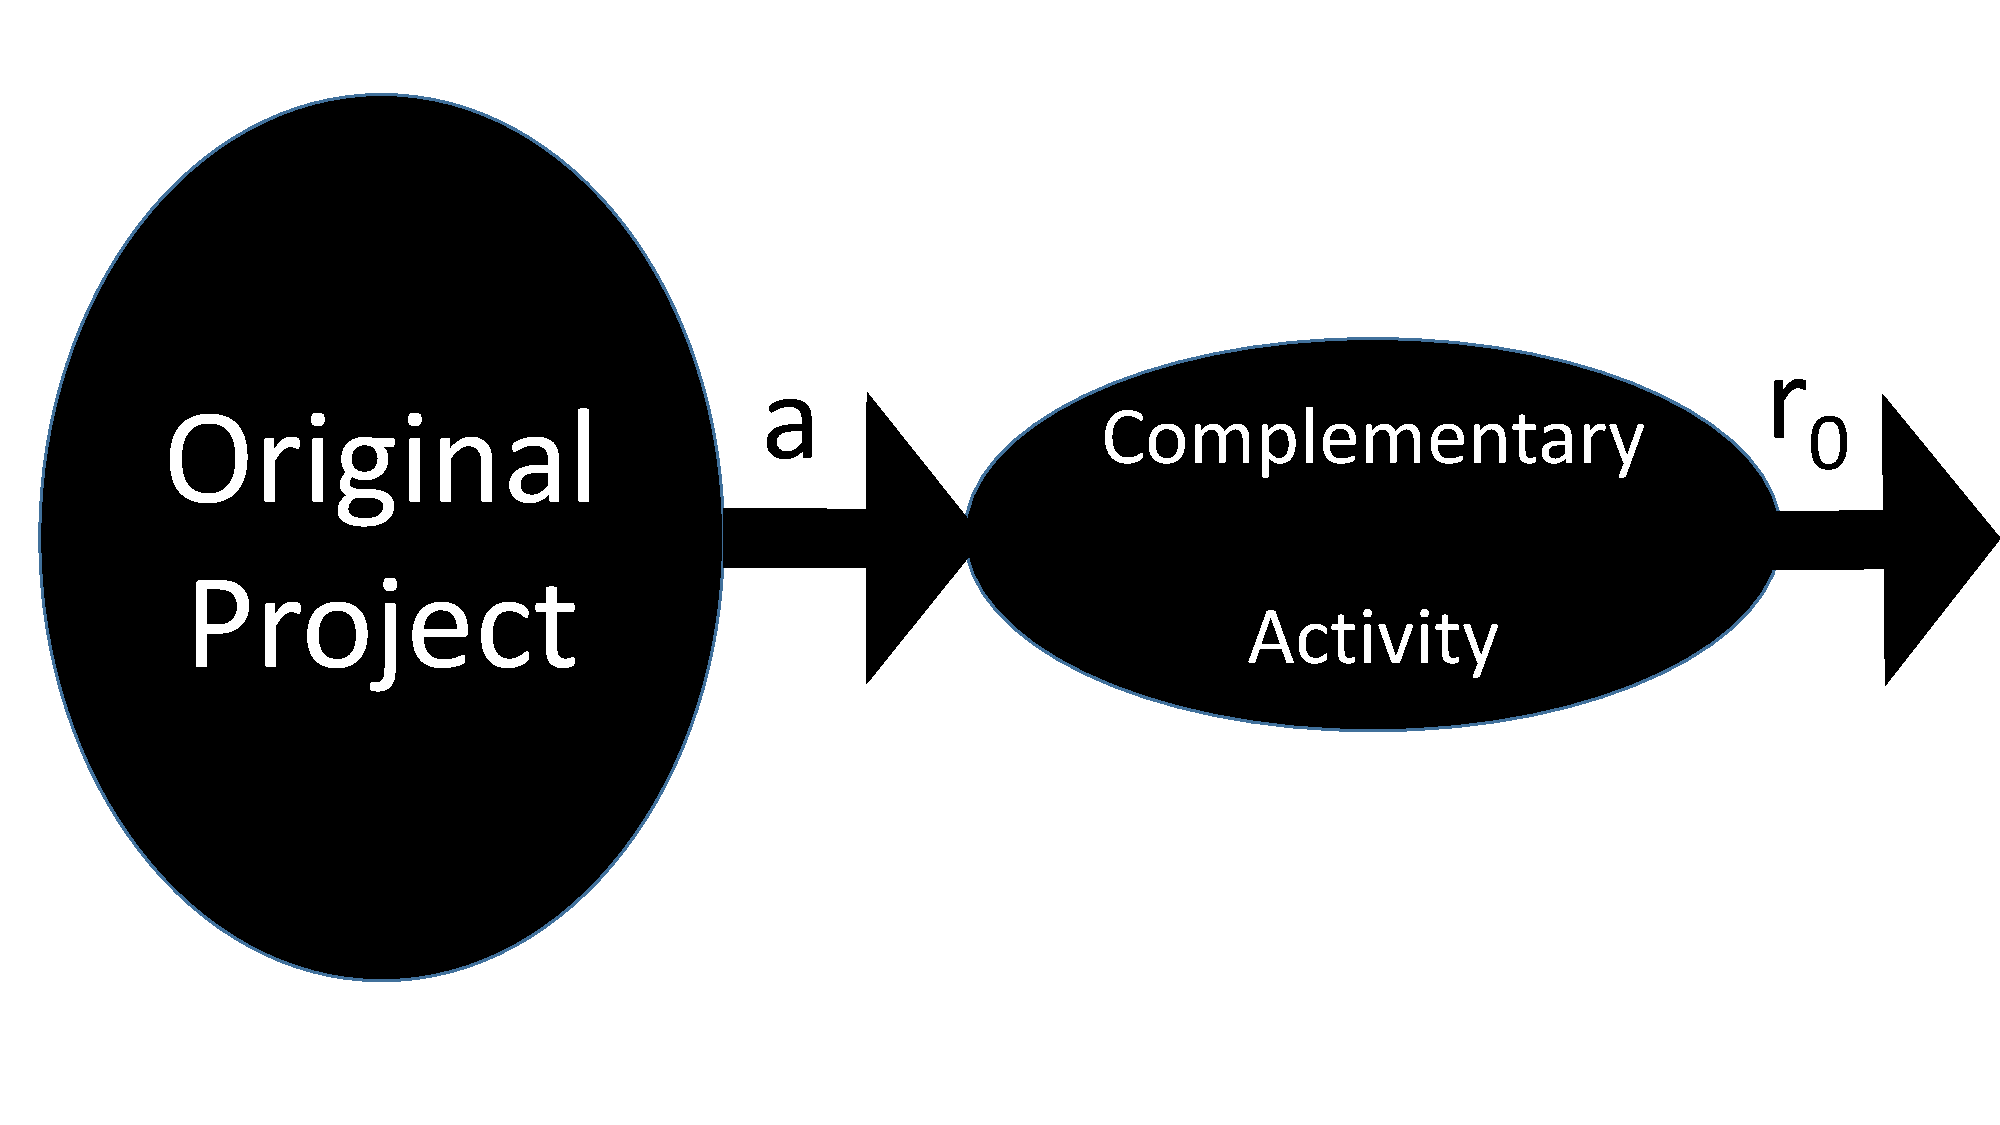
\includegraphics[scale=0.30]{uncertaindeadlines.pdf}
\caption{The Original Project embedded in the Manager's Project}
\label{fixXscaled}
\end{center}
\end{figure}
          Fortunately, the manager could simply re-define the actual project so that it finishes when the longer term project finishes.    This enlarged project will have the same required completion time $r_O$ as the stakeholder's long-term project.   The project network describing the new project consists of the network for the original project plus an additional activity, corresponding to the complementary activity, which can only start after all the activities in the original project have finished.  But while the manager may be able to affect the completion time of the activities in the original project by adding resources, the manager will not be able to affect the completion time of this complementary activity. \par
          If the completion time of the complementary activity is $t$ and if the actual completion time of the manager's project is $a$, then the completion time for the redefined project will be $a+t$.   The project will finish on time when $a+t \leq r_O$.    Because $t$ is uncertain, the project manager needs the stakeholder to specify an optimistic completion time, $t_O$, for the complementary project, as well as a pessimistic completion time $t_P$  and a most likely completion time, $t_L$.  Once $t_O$, $t_L$ and $t_P$ are specified, the manager can then use standard PERT-CPM methods to model the probability of the redefined project finishing by its new deadline $r_O$ (which is just the probability that $a+t \leq r_O$.)   The uncertainty in the deadline of the original project is completely determined by the uncertainty in the complementary activity.   (The uncertainty in the actual completion time, $a$, of the original project is, of course, described by the uncertainty in the activities within the original project.)  Since the manager is now responsible for a redefined project including the complementary activity, the manager will make decisions that appropriately recognize the uncertainty in the required completion time for the original project.
\subsection{Extension to General Projects}
          We now show how the solution for the special case just described can be extended to the more general case where there is no longer-term project but the stakeholder is still uncertain about the time when the project must finish.  Let $r_O$, $r_L$ and $r_P$ be the stakeholder's estimate of the latest possible project deadline, the most likely project deadline and the earliest project deadline.  Define $t=r_O-r$ where $r$ is the uncertain required completion time for the project.  Then $t$ will have a maximum possible (pessimistic) value of  $t_P = r_O-r_P$ , a most likely value of  $t_L = r_O-r_L$ and a minimum (optimistic) value of   $t_O = r_O-r_O=0$.  The manager's project will finish on time if $a < r $ (which implies $a+t < r_O$. )  Hence, making decisions to maximize the probability of $a+t$ being less than $r_O$ will be equivalent to making decisions to maximize the probability of the original project having a completion time, $a$, which is earlier than its original uncertain deadline, $r$.  \par
          To model this with the classical project management structure, i.e., an activity network, the manager re-defines the original project to have a deadline $r_O$ and to include a fictitious complementary activity with uncertain completion time $t$ which starts when all other activities finish.   Fictitious activities have been used, for other purposes, in other project management contexts (Vanhoucke (2013), pg. 244; Schwindt (2005), pg.8).  The classical project management solution to the original project supplemented with this added activity will be the appropriate solution to the original project where the stakeholder's completion time was uncertain.
\section{Why Ignoring Deadline Uncertainty Misleads Project Managers}
First consider the simplest case (CPM) with no uncertainty about the duration of each activity and the project manager ignoring deadline uncertainty by treating the deadline as if it equalled the median deadline.   Then if the manager scheduled activities to finish exactly at this estimated deadline, the project manager would conclude the probability of on-time completion was $100\%$ even though it was actually only $50\%$.  So ignoring deadline uncertainty can dramatically overestimate the on-time completion probability.\par
To consider the general case where there is uncertainty about project completion time,  let $X_i$ represent the uncertain completion time of path $i$ with $T$ representing the uncertain deadline.  This paper will use the term slack to describe $T-X_i$ which is the uncertain amount by which path $i$ finishes ahead of the deadline.  Let $e_i$ and $v_i$ be the mean and variance of this uncertain slack.  The probability of path $i$'s on-time completion is
$$ p_i= P(X_i \leq T) = P(T-X_i \geq 0) = P(\frac{T-X_i-e_i}{\sqrt{v_i}} \geq - \frac{e_i}{\sqrt{v_i}}) =
P(\frac{e_i-(T-X_i)}{\sqrt{v_i}} \leq \frac{e_i}{\sqrt{v_i}})  $$
Let $\eta_i=\frac{e_i-(T-X_i)}{\sqrt{v_i}}$ and $z_i=\frac{e_i}{\sqrt{v_i}}$ and let
$F_i$ be the cumulative distribution of $\eta_i$.  Then $p_i=P(\eta_i \leq z_i)=F_i(z_i)$. \par   
Suppose the manager who ignores the variance in the deadline estimates the deadline $t$ as the mean of $T_i$.  Then the mean value of $t-X_i$ is $e_i$ and the variance is $v^*_i<v_i$.    The manager will estimate the probability of on-time project completion as 
$$ p^*= P(\frac{e_i-(t-X_i)}{\sqrt{v_i}} \leq \frac{e_i}{\sqrt{v^*_i}})  $$
Let $\eta^*_i=\frac{e_i-(t-X_i)}{\sqrt{v^*_i}}$ and suppose that $\eta^*_i$ also has cumulative distribution $F_i$.   Then if $z^*_i= \frac{e_i}{\sqrt{v^*_i}})$, $p^*_i=F_i(z^*_i)$.  Then
\begin{itemize}
\item if $e_i>0$, then $z_i$ and $z^*_i$ are positive and $p_i=F(z_i) \leq F(z^*_i)=p^*_i$. Ignoring deadline uncertainty will lead to overestimation of path $i$'s probability of on-time completion.
\item if $e_i<0$, then $z_i$ and $z^*_i$ are negative and $p_i=F(z_i) \geq F(z^*_i)=p^*_i$. Ignoring deadline uncertainty will lead to underestimation of path $i$'s probability of on-time completion.
\end{itemize}
To adjust the probability of the project finishing on-time, the manager can reorganize specific activities by adding (or subtracting) resources from them.  When the manager adds resources, this is commonly referred to as the `crashing' decision.  Suppose the manager wishes to add just enough resources to increase path $i$'s on-time completion probability to equal some threshold $\alpha$.  Ignoring ignoring deadline uncertainty (when $e_i>0$) will lead the manager to add an insufficient level of resources and fall short of that goal.\par
But ignoring deadline uncertainty also distorts decisions about which path to crash.  Suppose the manager must choose between crashing path $i$ or path $j$ and always chooses to crash the path with the greatest schedule risk. For simplicity, suppose for this case only, that $F_i=F_j$.  
 Then the manager should crash path $i$ over $j$ if $$F_i(\frac{e_i}{\sqrt{v_i}}) \leq F_i(\frac{e_j}{\sqrt{v_j}}) \Longrightarrow \frac{e_i}{e_j} \leq \sqrt{\frac{v_i}{v_j}}$$
But the manager who ignores deadline uncertainty will crash $j$ over $i$ if  $\frac{e_i}{e_j} \geq \sqrt{\frac{v^*_i}{v^*_j}}$.
Thus the manager who ignores deadline uncertainty will make decisions contrary to the manager who recognizes requirement uncertainty when 
$$\sqrt{ \frac{v_i}{v_j}} \geq \frac{e_i}{e_j} \geq \sqrt{\frac{v^*_i}{v^*_j}}$$
If $v$ is the variance of deadline uncertainty, then this condition implies
$$ \frac{v^*_i+v}{v^*_j+v} \geq \frac{e^2_i}{e^2_j} \geq \frac{v^*_i}{v^*_j}   
\Longrightarrow   (1+\frac{v}{v^*_i})  \geq 1 + \frac{v}{v^*_j}  
\Longrightarrow  v^*_i \leq v^*_j $$
This shows that the manager who ignores deadline uncertainty will have a bias toward crashing paths with higher completion time variance. Hence ignoring deadline uncertainty overestimates project completion time and leads to inappropriate resource allocation decisions.
\section{Quantifying the Benefits of Recognizing Deadline Uncertainty}  
\subsection{Modeling Project Completion Time}
 To quantify the impact of these biases, number the paths in the project $i=1,...k$. 
 The probability of the project finishing on time is the probability that $T-X_i \geq 0, i=1,...,k$ which is the same as the probability
 $\eta_1,...\eta_k \leq z_1,...z_k$ . Let
 $F$ be the multivariate cumulative distribution of $\eta_1,....\eta_k$ so that the probability of on-time completion is
 $p=F(z_1,...,z_k)$. For the manager who ignores deadline uncertainty, the probability is
$p^*=F(z^*_1,....z^*_k)$. \par
Each path in the project is made of several activities, some of which may be shared by other paths.
Number the activities in the project $m=1,....M$ and let $\pi_m$ be the amount of resources associated with crashing activity $m$.   In some cases, crashing of an activity significantly reduces its completion time.  In other cases, it introduces confusion into the project and may significantly increase its completion times.  To model this, we assume \\
\bf Assumption 1: \rm Crashing activities $1...m$ while it reduces their mean duration will introduce uncertainties, uncorrelated with any other project uncertainties, which increase the variance of the activity's duration.  \\
Specifically suppose that optimally spending $\pi_1,...\pi_M$ on crashing activities $1,...m$ respectively reduces the mean duration by $x_1,....x_M$ respectively and increases the variance of duration by $\sigma^2_1,...\sigma^2_M$ respectively.
Let $I_{jm}=1$ if activity $m$ is on path $j$ with $I_{jm}=0$ otherwise. If $e^0_j$ and $v^0_j$ are the mean and variance of $T-X_j$ prior to crashing, then spending resources $\pi_1,...\pi_M$ on crashing leads to the following revised values of $e_j$ and $v_j$:
\begin{eqnarray*}
e_j &=& e^0_j+\sum_m x_m I_{jm}, j=1...k \\
v_j &=& v^0_j+\sum_m I_m \sigma^2_m, j=1...k
\end{eqnarray*}
Since $\sigma^2_m$ and $x_m$ are both increasing functions of only $\pi_m$, it is convenient to rewrite $\sigma^2_m$ as only a function of $x_m$.   As a result, the problem of choosing $\pi_1,...\pi_M$ to maximize the on-time completion probability can be rewritten as the problem of choosing $x_1,....x_M$ to maximize $\ln(p)$.\par 
 The first-order Kuhn-Tucker conditions for $x_1,...x_M$ are
$$\frac{\partial \log p}{\partial x_m} = \sum_{j=1}^k \frac{\partial \log F(z_1,...z_k)}{\partial z_j} 
\frac{\partial z_j}{\partial x_m} =0  , m=1,...M $$
where
$$ \frac{\partial z_j}{\partial x_m} = \frac{1}{\sqrt{v_j}} \frac{\partial e_j}{\partial x_m}-  
\frac{1}{2} e_j v_j^{3/2} \frac{\partial v_j}{\partial x_m}]  \mbox{ and } \frac{\partial e_j}{\partial x_m}=1  $$
Note that all $M$ equations are satisfied if it is possible to choose $x_m$ so that
\begin{equation} 
\frac{\partial z_j}{\partial x_m} = (1/\sqrt{v_j}) [1 -   \frac{e_j}{2 v_j}  \frac{\partial v_j}{\partial x_m}] =
\frac{v_j^{-3/2}}{2}[2v_j - e_j \frac{\partial v_j}{\partial x_m}  ] 
 \label{firstorder}
\end{equation}
\subsection{Second-order Optimality Conditions}
The first-order condition will only define an optimal solution if the second-order condition is satisfied.
Three assumptions will be made to ensure the second-order condition is satisfied.  The first assumption is: \\
\bf Assumption 2: \rm The coefficient of variation of the uncertainty induced by crashing activity $m$ is some constant $s_m$ independent of $x_m$ which may vary from activity to activity \\ 
Then 
$\frac{\sigma_m}{x_m}=s_m$, $\sigma^2_m=x^2_m s^2$ and $\frac{\partial v_j}{\partial x_m} = 2 x_m s^2$.  Substituting into the first-order conditions gives
\begin{eqnarray*}
\frac{\partial z_j}{\partial x_m} &=& \frac{v_j^{-3/2}}{2}[2v_j - e_j \frac{\partial v_j}{\partial x_m}] \\ &=&
\frac{v_j^{-3/2}}{2}[2v^0_j + 2 \sum_m I_{mj} x^2_m s^2 -  (e^0_j + \sum_m I_{mj} x_m) 2 x_m s^2_m)]  \\
&=& v{j^{-3/2}} [v^0_j-x_m s^2_m e^0_j] 
\end{eqnarray*}
which is satisfied if 
$$ x_m =   \frac{ v^0_j}{s^2_m e^0_j}  $$
So the mean reduction in activity $m$ when the mean completion time is large (and $e^0_j$ is smaller), when the variance of the activity is large and when the uncertainty induced by crashing is smaller.   \par
The second assumption made to ensure concavity is:
\\ \bf Assumption 3: \rm  $\ln(p)$ is concave in $z_1,...z_k$. \\
 This assumption will be true for log-concave densities like the normal distribution, extreme value distribution, the Laplace distribution, the logistics distribution, the uniform and exponential distribution as well as for many other distributions whose density is not log-concave (or are only log-concave for certain parameter settings.) \par
Assuming $\ln(p)$ is concave in $z_1,...z_k$ does not imply it is concave in $x_1,...x_k$. \par  To ensure that $ln(p)$ is concave in $x_1,...x_k$, this paper will additionally require that the Hessian matrix $\frac{\partial^2 z_j}{\partial x_m \partial x_{m*}} \geq 0$, be negative definite.   To determine the circumstances under which this condition is satisfied, define 
$A_j=[v^0_j - x_m s^2_m e^0_j] $ so that $\frac{\partial z_j}{\partial x_m} = v_j^{-3/2} A_j $.  Then
$$\frac{\partial^2 z_j}{\partial x_m \partial x_{m*}} =  \frac{\partial v_j^{-3/2}}{\partial x_{m*}} A_j +
 v_j^{-3/2} \frac{\partial A_j}{\partial x_{m*}}  $$
Evaluating this derivative at the point where the first-order condition is satisfied gives
$$
\frac{\partial^2 z_j}{\partial x_m \partial x_{m*}} = v_j^{-3/2}\frac{\partial A_j}{\partial x_{m*}} 
=  - s^2_m e^0_j \mbox{ for } m=m^* \mbox{ and } = 0  \mbox{ for } m \neq m^* $$
      If $e^0_j \geq 0$,  then the diagonal elements of the matrix, $\frac{\partial^2 z_j}{\partial x^2_m} $ is negative while the off-diagonal elements equal zero.  Hence the matrix is negative definite and the second-order condition is satisfied if we this third assumption: \\
      \bf Assumption 4: \rm  Prior to crashing, the mean duration of each path is less than the mean deadline ($e^0_j \geq 0$).   \\
If this condition were not true, then the project prior to crashing would --- in the absence of uncertainty in both deadlines and activity durations --- always run late.  In our view, it is not unreasonable to rule out such a possibility.    
\par
Since the concavity conditions are satisfied, the solution of the first-order conditions,
\ref{firstorder}, $x_m=\frac{v^0_j}{s^2_m e^0_j}$ is an optimum.
\subsection{Computation of Schedule Risk}
The first-order conditions imply $$e_j=e^0_j+\sum_m I_{mj} x_m = e^0_j +\frac{v^0_j}{e^0_j} \sum_m \frac{I_{mj}}{s^2_m} $$
Define $a_j=\sum_m \frac{I_m}{s^2_m}$ so that $$e_j=e^0_j + \frac{v^0_j}{e^0_j} a_j$$. In addition
$$ v^0_j + \sum_m I_{mj} (x_m s_m)^2 = v^0_j + \sum_m I_{mj} (\frac{v^0_j}{s^2_m e^0_j} s_m)^2 =
v^0_j + (\frac{v^0_j}{e^0_j})^2 \sum_m \frac{I_{mj}}{s^2_m} $$ so that
$$v_j= v^0_j + (\frac{v^0_j}{e^0_j})^2 a_j $$ 
Then
\begin{eqnarray*}
z_j &=& \frac{e^0_j + \frac{v^0_j}{e^0_j} a_j}{\sqrt{v^0_j+(\frac{v^0_j}{e^0_j})^2 a_j }} 
= \frac{\frac{e^0_j}{\sqrt{v^0_j}} + \frac{(v^0_j)^{1/2}}{e^0_j} a_j}{\sqrt{1+ \frac{v^0_j}{(e^0_j)^2} a_j }} 
= \frac{ z^0_j + \frac{a_j}{z^0_j}}{\sqrt{1+ \frac{a_j}{(z^0_j)^2}}}  \\
&=& z^0_j \frac{1 + \frac{a_j}{(z^0_j)^2}}{\sqrt{1+ \frac{a_j}{(z^0_j)^2}}} 
= z^0_j \sqrt{1 + \frac{a_j}{(z^0_j)^2}}   
=   \sqrt{(z^0_j)^2 + a_j}
\end{eqnarray*}
with the on-time completion probability for a manager who recognizes deadline uncertainty being  
$p=F(z_1,...z_k)$ using, for example, the technique described in the first two sections of this paper.  \par  
Now consider the manager who ignores deadline uncertainty
 Let $\kappa=
\frac{v^*_j}{v^*_j+v}$ so that $1-\kappa$ represents the fraction of the variance in $T-X_j$ neglected by the manager who ignores deadline uncertainty.   This manager sets the mean reduction in activity $m$' duration to be
$$x^*_m=\frac{v^*_j}{s^2_m e^0_j}=\frac{v^*_j}{v^0_j} \frac{v^0_j}{s^2_m e^0_j} =  \kappa x_m < x_m$$
As a result, 
\begin{eqnarray*}
e^*_j &=& e^0_j+\kappa \sum_m I_{mj} x_m = e^0_j + \kappa a_j \frac{v^0_j}{e^0_j} < e_j \\
 v^*_j &=& v^0_j + \sum_m I_{mj} (\kappa x_m s_m)^2 = v^0_j + \kappa^2 a_j (\frac{v^0_j}{e^0_j})^2 < v_j 
 \end{eqnarray*}
 Then
\begin{eqnarray*}
z^*_j &=& \frac{e^0_j + \kappa \frac{v^0_j}{e^0_j} a_j}{\sqrt{v^0_j+\kappa^2(\frac{v^0_j}{e^0_j})^2 a_j }]} 
= \frac{ z^0_j + \kappa \frac{a_j}{z^0_j}}{\sqrt{1+ \kappa^2 \frac{a_j}{(z^0_j)^2}]}}   \\
&=& z^0_j \frac{1 + \kappa \frac{a_j}{(z^0_j)^2}}{\sqrt{1+ \kappa^2 \frac{a_j}{(z^0_j)^2}]}} 
=  \frac{(z^0_j)^2 + \kappa a_j}{\sqrt{(z^0_j)^2+ \kappa^2 a_j }}  
\end{eqnarray*}
 Note that $z_j \geq z^*_j$ when 
 $$\sqrt{(z^0_j)^2+a_j} \geq \frac{(z^0_j)^2 + \kappa a_j}
 {\sqrt{(z^0_j)^2+\kappa^2 a_j}}  \Longrightarrow ((z^0_j)^2+ a_j) ((z^0_j)^2 + \kappa^2 a_j) \geq ((z^0_j)^2 +\kappa a_j)^2  \geq 0 $$
This is true if and only if 
\begin{eqnarray*}
(z^0_j)^4 &+& (z^0_j)^2 (a_j + \kappa^2 a_j) + \kappa^2 a^2_j - [(z^0_j)^4 + 2 (z^0_j)^2 \kappa a_j + \kappa^2 a^2_j] \\ &=& 
  (z^0_j)^2 a_j[(1 + \kappa^2 ) - 2 \kappa] 
  =  (z^0_j)^2 a_j(1-\kappa)^2 \geq 0 
  \end{eqnarray*}
which is always true.  Hence $z_j \geq z^*_j$ and $p=F(z_1,...z_k) \leq p^*=F(z^*_1,...z^*_k) $.  Ignoring deadline uncertainty reduces the project's on-time completion probability. \par
Since both $\kappa$ and $z^0_j$ depend on $v$,   it is useful to define $$z^1_j=\frac{x_j}{\sqrt{v^*_j}}=
\frac{x_j}{\sqrt{v_j \kappa_j}} = \frac{z^0_j}{\sqrt{\kappa_j}} $$ 
which is independent of $v$.   Then 
\begin{eqnarray*}
z_j &=& \sqrt{\kappa_j(z^1_j)^2 + a_j} \\
z^*_j &=&  \frac{ \kappa[(z^1_j)^2+ a_j]}{sqrt{ \kappa[(z^1_j)^2 + \kappa a_j]}} \\  
&=& \sqrt{\kappa} \frac{(z^1_j)^2+ a_j}{\sqrt{(z^1_j)^2 + \kappa a_j}}  
\end{eqnarray*}
so that $z_j,z^*_j$ are functions of $\kappa$ (which measures relative deadline variance), $a_j$ (which measures the ease of crashing path $j$) and $z^1_j$ (which measures all other path attributes.\par
The improvement in on-time completion probability resulting from recognizing deadline uncertainty is $p-p^*$.  When deadline variance is small and $\kappa \approx 1$, $z_j \approx z^*_j, j=1...k$.  When deadline variance is large and $\kappa \approx 0$, $z^*_j \approx 0$ and $z_j=\sqrt{a_j}, j=1...k$.      
\section{Generality of this Approach}
This approach was designed to supplement those project management techniques which presume that the project deadline is fixed.  Our innovation is in showing how uncertain deadlines could be easily integrated into such methods using a dummy activity.  Because PERT is the most well-known example of such a method,  this paper focused on PERT.  But PERT makes many other assumptions which have been criticized.  As this section notes, the benefits of our approach are not contingent on these PERT assumptions being satisfied. \par
Consider first the limitations in PERT's objective function.  PERT focuses on maximizing the probability of finishing the project by the deadline.  But there are many other objectives e.g., the minimization of expected project completion time, the minimization of a weighted average of mean completion time and the variance of completion time, value at risk, etc.   However the results of this paper can be used to enable PERT to maximize the expected utility of completion time for any well-defined Von Neumann-Morgenstern utility.  Specifically, any 
von Neumann-Morgenstern utility can always be interpreted as the cumulative distribution of some possibly latent random variable.  As a result, maximizing  expected utility is equivalent to maximizing the probability of completion time exceeding this latent random variable. If this latent random variable is interpreted as an uncertain deadline, then the methodology in this paper addresses any PERT problem where the objective function is defined by a utility function.\par
Next consider PERT's assumption that the critical path completion time is normally distributed.  While this assumption has some plausibility when the number of activities is large and the correlation between paths is small, there are many realistic examples for which this assumption is inappropriate.  The proposed method of adding a complementary dummy activity does not place any limitation on the distribution used to model path completion times.  And, in fact, the analytic demonstration of the benefits of this approach first focused on the broader family of two parameter distributions before focusing on the normal distribution to develop analytically tractable estimates of the benefits of the method.  But while normality assumptions may be useful in calculating the benefits of this approach, they are not required to achieve the benefits of this approach.\par
 While PERT recognizes that some activities may need to be finished before other `precursor' activities can start, it is not structured to address activities with cyclic dependencies (where one activity requires inputs from a second activity and the second activity provides inputs to the first activity).  Fortunately the design structure matrix methods (Eppinger and Browning, 2012) do address this limitation by showing how cyclic dependencies can be eliminated with typically minimally  adverse impact on the project.  Our approach makes no contribution to this particular problem and assumes that techniques like the design structure matrix have already been used to eliminate cyclic dependencies. \par
PERT assumes each activity will start as soon as all precursor activities are finished.  But if the start of this new activity will monopolize equipment needed by an activity that starts later, starting each activity as soon as possible may delay the project's completion time.  Since this paper shows how our approach can improve resource-allocation decisions (like crashing), the proposed method is potentially useful in these more complex decisions.  \par
Finally PERT assumes project completion time is determined by the completion time of the critical path.  Since the proposed approach creates a complementary activity which starts after every activity is finished, the value of the proposed approach is unaffected by which path actually finishes last. Note also that the family of distributions included in our analysis of the benefits of this approach includes the Gumbel which does describe the asymptotic distribution of the maximum of many path completion times. In fact, if $X$ and $T$ both have Gumbel distributions, their difference is a logistic distribution which is also among the family of distributions considered in our analysis.
Hence our approach is valid even when PERT's critical and distributional assumptions are violated.  \par
But while the validity of our methodology is unaffected by the common limitations associated with PERT, its simplicity makes it especially useful for commonly used network-based methods like PERT.   But there are alternative more complex methods for allocating time and resources to activities.
Stochastic programming based optimization is generally a preferred method for identifying strategies acceptably close to optimal in an acceptable computation time. For example, Resource Constrained Project Scheduling Problems (RCPSP, e.g., Brucker et al, 1999) is a relatively sophisticated method which typically minimizes the expected time to completion (although the literature discusses other possible objectives, e.g. value-at-risk.) Once a problem is thus formulated, it would require little additional effort to instead maximize the probability of meeting a given deadline (or similarly value-at-risk minimization), and even to add an additional dummy uncertain variable for the deadline.   Hence the incremental contribution of the proposed approach to these methods is much smaller than its contribution to methods like PERT or GERT.  \par
But because these methods are harder for most project managers to use,  there is a significant cost to using these methods versus PERT or GERT.  Hence evaluating our approach versus these more complex approaches involves a cost/benefit analysis of how well our enhancement of PERT performs compared to more difficult, but higher performing, stochastic optimization methods.  The next section focuses on this question. 
\section{Simulation Comparison of Alternate Approaches}
There is a trade-off between the ease of implementation and benefit of modified-PERT compared to that for more modelling intensive approaches. Of course, if the project conforms exactly to the assumptions of modified-PERT, additional modelling efforts will not produce any benefit. To explore the usefulness of the proposed approach extends to other situations, we consider a slightly more complicated activity network and simulate in Microsoft Excel the performance of the PERT heuristic against an optimization approach under different assumptions about uncertainty.  \par
Specifically, we consider the activity network shown in Figure $4$, which is a tree with one level of branches of varying lengths beyond the root.
\begin{figure}[h]
\begin{center}
\includegraphics[scale=0.30]{uncertaindeadlinestwo.pdf}
\caption{The Project Network}
\label{fixXscaled}
\end{center}
\end{figure}
 This is still relatively simple, but different enough from a linear project to test whether the results are an artifact of the critical path assumption. The sequence of activities $1, 2$ and $3$ forms the first branch, activities $4$ and $5$ in sequence form the second, and activity $6$ is the third. All three branches precede activity $7$. We select initial parameters so that
\begin{itemize} \item the mean deadline is greater than the mean project completion time;
\item it is plausible that some activity not on the PERT critical path will delay completion; 
\item there is a non-trivial chance that the project will not be on time. 
\end{itemize}
We initialize random variables $Y_i$ for the activity durations with means $m_i'$  of $6, 5, 4, 8, 6, 13$ and $8$ respectively, each with the same initial standard deviation $S_i’ = S$ (which is varied across four scenarios). The project deadline $T$ is uncertain with mean $25$ and standard deviation $3$.  The effect of crashing activity $i$ is to reduce its mean to $m_i'' \geq 0$, and to increase its standard deviation to $S_i’’ = S + (m_i'-m_i'')$. A crashing strategy, which leads to reductions in the mean time for each activity, creates a new set of random variables $Y’’. Y$ and $T$ which are Gaussian and independent.
To calculate the probability of on-time completion, we first compute the cumulative density function for $\chi =  \max(Y_1 + Y_2 + Y_3, Y_4+Y_5, Y_6)$, which is defined by 
$$\Pr.\{ \chi \leq w) =  \Pr.\{Y_1 + Y_2 + Y_3 \leq w) \Pr.\{Y_4 + Y_5\leq w) \Pr.\{Y_6 \leq w \},$$ noting that the sum of activity times on each branch is Gaussian with mean equal to sum of the activity means and variance equal to the sum of activity variances on that branch. The project is on time if $\chi + Y_7 <= T$, i.e., if $ \chi < T-Y_7$ where $T-Y_7$ is the difference between two Gaussian random variables and hence is Gaussian. (This is equivalent to adding the dummy activity for deadline uncertainty.) From the joint distribution of $\chi$  and $T-Y_7$, we obtain the density $\Phi(T - Y_{7} - \chi) $ and thus $\Pr.\{ T - Y_{7} - \chi \geq 0\}$, i.e. the probability the project finishes by its deadline. 
We then use a generalized reduced gradient algorithm to solve for the crashing strategy which maximizes this probability for given parameters of $Y''$ and $T$, subject to the constraint that each $m''_i \geq 0$. We do this once for the scenario in which initial activity times are known so that $S = 0$, once where activity times have low uncertainty ($S = 0.5$), once with medium uncertainty ($S = 1.0$), and once with high uncertainty ($S = 2.0$). \par
For each scenario, we identify the strategy which optimizes probability of success under four different assumptions about uncertainty:
\begin{enumerate}
\item PERT: The deadline is assumed to be fixed with standard deviation $0$, and there is no chance that activities $4, 5$ or $6$ can enter the critical path (i.e., they are assumed to have means of $0$ and standard deviations of $0$);
\item Optimization: The deadline is fixed but all activities might be appear on the critical path and therefore all might be crashed, i.e., the correct parameters are entered;
\item Enhanced PERT: The deadline is assumed to have its correct standard deviation of $3$, but as before activities off the initially identified critical path $(1,2,3, 7)$ are ignored; 
\item Enhanced optimization: all activities are crash-able and deadline uncertainty is included.
\end{enumerate}
 Note that strategies $(1), (2)$ and $(3)$ are optimal under conditions which somehow distort the project, while strategy $(4)$ is a gold-standard which is optimal under the correct assumptions. Our measure of performance is the probability that each of the strategies thus identified leads to on-time completion under the assumptions of $(4)$. For additional comparison, the table includes the probability of success if there no crashing. 
The results in Table $1$, as expected, show that no crashing is worst and enhanced optimization is best in each scenario. 
\begin{table}
        \centering
        \begin{tabular}{ |c||  c | c | c | c | c | } \hline   
       & No Crashing & PERT & Optimization &  Enhanced  PERT & 
       Enhanced  Optimization   \\
       \hline
      S=0.0  & 74.21 $\% $ & 74.21 $\%$ & 74.21 $\%$ & $91.24 \%$ & $94.49 \%$ \\
       S=0.5 & $72.1 \% $ & $85.47 \%$ & $77.82 \%$ & $88.29 \%$ & $91.07 \%$ \\
       $S=1.0$   & $66.18 \% $ & $82.81 \%$ & $81.29 \%$ & $84.65 \%$ & $87.91 \%$  \\
       $S=2.0$   & $53.83 \% $ & $77.25 \%$ & $81.49 \%$ & $77.29 \%$ & $81.50 \%$  \\
       \hline
           \end{tabular}
         \caption{Outcomes of Simulation Experiment}
         \end{table} 
For $S \leq 1.0$, the performance of enhanced PERT is close to the performance of enhanced optimization with both enhanced PERT and enhanced optimization substantially outperforming both PERT and optimization.  When $S = 2.0$, the deadline uncertainty is small relative to the project duration uncertainty and optimization, with or without enhancement, outperforms both PERT and enhanced PERT.\par
Also note that for
$S=0.5$ and $1$, PERT counter-intuitively performs better than optimization because 
\begin{itemize}
\item the risk aversion of the project manager in a favourable situation is artificially strengthened when deadline uncertainty is ignored which leads to too little crashing on any of the three branches
\item PERT ignores the possibility that any activities will be replaced on the critical path, and so overweights the impact of crashing those activities.  This offsets the bias the risk-aversion created by ignoring deadline uncertainty
\end{itemize}
 In practical terms, when the scale of the project is not so large or structure of the project is not so complex as to justify large modelling expense, project managers can still obtain considerable benefit utilizing internal staff to conduct modified-PERT analysis in problems involving substantial deadline uncertainty.
\section{Summary}
Many projects must be completed in the presence of uncertainty about when the stakeholder requires the project to be finished.    In order to apply PERT (or GERT), project management currently requires that the project manager assume a fixed required project completion time, until such time as it is formally modified by a change control process.   In other words, the project manager is required to ignore the uncertainty in the project completion time until such time as the change control process modifies that completion time.  There is considerable evidence that this is a sub-optimal way to address uncertainty.  As this paper shows, this deficiency can be corrected by simply supplementing the initial list of project activities with a fictitious dummy activity with the same uncertainty as currently exists in the deadline. The deadline for the supplemented project is an optimistic estimate of the uncertain deadline.  Managing this supplemented project appropriately using standard methods of project management then appropriately accounts for the uncertainty in the deadline.\par
This paper then examined the potential benefit of this innovation in making project crashing decisions. This paper considered the case in which project crashing could reduce project completion time by a fixed amount without any change in project uncertainty.  But we also considered models in which either the standard deviation or the variance of project completion time increased linearly with the expected reduction in project completion time.   In all of these cases, it was assumed that these plans had been pre-screened to eliminate crashing plans which were dominated by other existing plans.  To facilitate the analysis, it was assumed that the difference between deadline and project completion time was described by a two-parameter distribution with centering and scaling parameters.  But for analytic simplicity, actual computation of the value of considering uncertainty (versus ignoring it) was made assuming this difference was normally distributed.  Because of its convenience and its asymptotic justification by the central limit theorem, virtually all PERT applications make this assumption. Nonetheless consideration of more general distributions is important because project completion time, instead of being the sum of the duration of independent activities is the maximum completion time of multiple potentially highly correlated paths.  These analyses do establish that there is often a substantial benefit from recognizing deadline uncertainty.\par
This leads to an enhancement of PERT and related project management tools.   This paper compared enhanced PERT with the optimal solution (based on generating and comparing all possible crashing plans.) and found that when deadline uncertainty was significant relative to project uncertainty, enhanced PERT significantly outperformed PERT and performed almost as well as the optimal crashing plan.   Because of the expertise involved in using stochastic optimization to achieve near-optimal crashing plans, this enhancement provides an attractive alternative to near-optimal crashing plans for the widespread community of project managers. \par
In summary, the key contribution of this paper was to introduce the new
and somewhat counter-intuitive idea of recognizing the uncertainty in the project deadline by introducing an artificial activity.  In the context of PERT (and related network descriptions of projects), this way of recognizing deadline uncertainty requires only minimal changes in existing methodologies.  This paper introduced this idea and estimated its potential improvement in existing project management practices.
\begin{thebibliography}{10}
\bibitem{bbb} Brucker, P., A. Drexl, R. Mohring, K. Neumann, and E. Pesche (1999). Resource-constrained project scheduling: Notation, classification, models,
 and methods. {\em European Journal of Operational Research}. 112. 3-41
  \bibitem{a} Calhoun, K., R. Deckro, J. Moore, J. Chrissis and J. Van Hove. (2002). Planning and re-planning in project and production scheduling. {\em Omega.} 30, 155-170.
  \bibitem{b}	Chapman, C and S. Ward. (1997). {\em Project Risk Management: Processes, Techniques and Insights.} Wiley, New York
  \bibitem{c}	Clemen, R. (1996). {\em Making Hard Decisions.} 2nd ed. Duxbury Press, Belmont, MA.
  \bibitem{cc}  Creemers, S., B. De Reyck and R. Leus (2015). Project planning with alternative technologies in uncertain environments. {\em European Journal of Operational Research.} 242(2), 465-476.
  \bibitem{d}	Ding, C. and Y. Zhu.(2015). Two empirical uncertain Models for project scheduling problem. {\em Journal of the Operational Research Society.} 66, 1471-1480.
 \bibitem{e}	Elmaghraby, S. (2005). On the fallacy of averages in project risk management. {\em European Journal of Operational Research.} 165, 307-313.
 \bibitem{est}  Estevez-Fernandez, A. (2012).  A game theoretical approach to sharing penalties and rewards in projects. {\em European Journal of Operational Research.} 216(3), 647-657.
   \bibitem{f}	Golenko-Ginzburg, D. (1989). PERT assumptions revisited.{\em Omega} 17, 393-396.
  \bibitem{g}	Herroelen, W. and R. Leus (2005). Project scheduling under uncertainty: Survey and research potentials. {\em European Journal of Operational Research.} 165. 289-306.
  \bibitem{h}	Herroelen, W. and R. Leus (2003). The construction of stable project baseline schedules. {\em European Journal of Operational Research.} 156. 550-565.
  \bibitem{hh}  Hu, X., N. Cui, E. Demeulemeester, and L. Bie (2016). Incorporation of activity sensitivity measures into buffer management to manage project schedule risk. {\em European Journal of Operational Research}, 249(2), 717-727.
  \bibitem{j}	Huemann, M., R. Turner and A. Keegan (2007). Managing human resources in the project-oriented company. In Morris, P and J. Pinto. {\em The Wiley Guide to Project Organization and Project Management Competencies.} John Wiley \& Sons: Hoboken, New Jersey
  \bibitem{k}	Kamburkowski, J. (1996). New validations of PERT times.  {\em Omega}, 25(3) 323-328.
  \bibitem{l}	Keisler, J. and R. Bordley. (2015). Project management decisions with uncertain targets. {\em Decision Analysis.} 12, 1, 15-28.
  \bibitem{keefer} Keefer, D. and W. Verdini (1993). Better estimation of PERT activity time parameters. {\em Management Science.} 39, 9, 1086-1091.
  \bibitem{m}	Kerzner, H.  (2009)  {\em Project Management: A Systems Approach to Planning, Scheduling and Controlling.} John Wiley \& Sons: Hoboken, New Jersey
  \bibitem{n}	Khodakarami, V., N. Fenton and M. Neil. (2007). Project scheduling: Improved approach to incorporate uncertainty using Bayesian networks. {\em Project Management Journal.} 38(2),  39-49.
  \bibitem{o}	Klastorin, Ted (2003). {\em Project Management: Tools and Trade-offs} (3rd ed.). John Wiley \& Sons: Hoboken, New Jersey.
  \bibitem{p}	Maylor, H., R. Vidgen and S. Carver (2008). Managerial complexity in project-based operations: A grounded model and its implications for practice.  {\em Project Management Journal.} 39(S1), S15-S26.
  \bibitem{r}	Meredith, J., S. Mantel (1995). {\em Project Management: A Managerial Approach.} John Wiley and Sons, Hoboken: New Jersey
  \bibitem{s}	Miller, R. (1963). {\em Schedule, Cost and Profit Control with PERT.} McGraw-Hill, New
              York.
  \bibitem{t} Morgan, M. and M. Henrion (1992). {\em Uncertainty: A Guide to Dealing with Uncertainty in
  Quantitative Risk and Policy Analysis.}  Cambridge University Press:Cambridge, U.K.
  \bibitem{neu}  Neumann, J. and J. Zimmerman (1999).  Resource leveling for projects with schedule-dependent windows.  {\em European Journal of Operational Research.}  117(3), 591-606.
  \bibitem{tt} Pérez, J. G., M.Martín, C. García and M. Granero (2016). Project management under uncertainty beyond beta: The generalized bicubic distribution. {\em Operations Research Perspectives} 3, 67-76.
  \bibitem{u} Pich, M. ,C.Loch and A. DeMeyer. (2002). On uncertainty, ambiguity, and
  complexity in project management. {\em Management Science}, 1008-1023, 48,8
  \bibitem{v} Project Management Institute (2013). {\em A Guide to the Project Management Body of
  Knowledge} (5th ed.). Project Management Institute.
  \bibitem{w} Schwaber, K.  (2004). {\em Agile Project Management with SCRUM.} Microsoft Press,
           Redmond, Washington
  \bibitem{x} Schwindt, C. (2005). {\em Resource Allocation in Project Management.} Springer: New York
  \bibitem{y} Sculli, D. (1989). A historical note on PERT times. {\em Omega} 17(2), 195-196.
  \bibitem{z} Vanhoucke, M. (2013). {\em Project Management with Dynamic Scheduling.} Springer, New
          York.
  \bibitem{ab} Ward, S. and C. Chapman.(2003). Transforming project risk management into project
          uncertainty management. {\em International Journal of Project Management}, 21, 97–105
  \bibitem{ac} Zafra-Cabeza, A., M. Ridao and E. Camacho. (2008). Using a risk-based approach to
         project scheduling: A case illustration from semiconductor manufacturing. {\em European
        Journal of Operational Research.} 190, 708-723.
  \end{thebibliography}
\end{document}

\par
But this formulation assumes that the crashing budget is unlimited.   If there were a reward $R$ for successful project completion with the costs of crashing  being $\sum_{j=1}^k \pi_j$, then the first-order conditions are
$$R \frac{\partial p}{\partial \pi_m} =1   \Longrightarrow 
\frac{\partial \log p}{\partial \pi_m} = \frac{1}{Rp}  \Longrightarrow
\sum_{j=1}^k \frac{\partial \log F(z_1,...z_k)}{\partial z_j} 
\frac{\partial z_j}{\partial \pi_m} =\frac{1}{pR}  $$
A variation on this formulation maximizes $p$ subject to a budget constraint.    It leads to these same first-order conditions with $\frac{1}{pR}$ replaced by the Lagrangian multiplier associated with the budget constraint.  But for simplicity, the simulation only considers the case where $\frac{1}{pR}$ is approximately zero.    To supplement this theoretical demonstration, a later section randomly simulates actual project networks.   This second simulation will show that our claimed benefits are still substantial even in realistic settings where crashing alters the correlation among paths.\par
Note that much of this analysis,  done where $e$ and $sqrt{v}$ represented means and standard deviations, could be generalized to the case where $e$ and $\sqrt{v}$ represent the centering and scaling parameters for two-parameter distributions.  
\end{document}  
\section{The Efficient Frontier}
Let $X$ be the maximum of $X_1,...X_k$ with $v^*$ being the variance of $X$.  Then $p$ is the probability that $T-X \geq 0$.  Let $e$ be the mean $T-X$ with $v+v^*$ being its variance.  Let $\eta=\frac{e-(T-X)}{\sqrt{v+v*}}$ and 
let $F_0$ be the cumulative distribution function of $\eta$.  Then the probability that
$T-X \geq 0$ is the probability that $\eta \leq z$ and $p=F(z)$. \par
 Different crashing decisions lead to potentially different values of $v^*$ and $e$.  If these values are plotted for each alternative crashing plan, the set of points will be bounded by an efficient frontier.  For all the crashing plans which lead to some value $e$, there is some optimal value of $v^*$ leading to the highest project completion time probability, i.e., the probability that the project will be completed on time. For the values of $e$ and $s$ on the efficient frontier, $v^*$ is a function of $e$. 
 To choose $e$ to optimize $p$, set the derivative of $F(z)$ with respect to $e$ to zero to get
      $$\frac{\partial F}{\partial e} = \frac{\partial \Phi}{\partial z} \frac{\partial z}{\partial e} =0 $$
      Since $\frac{\partial F}{\partial z}$ is never zero, $\frac{\partial F}{\partial e} =0$ implies
      $$\frac{\partial z}{\partial e} =( \frac{1}{\sqrt{v^s^2+V}} - \frac{e \frac{\partial v*}{de}}{(v^*+V)^{3/2}}) = 0 $$
      which implies that at the optimum $e_U$ and $v^*_U$,
      \begin{equation}
    (v^*_U+v) = \frac{\partial v*_U}{\partial e_U} e_U
      \end{equation}
    Appendix B specifies the conditions required to ensure that this is a global optimum when $e>0$. \par 
When these conditions are satisfied, the manager who recognizes requirement uncertainty (as recommended in the approach proposed in this paper) will choose the value of $e_U$ (and the corresponding value of $s_U$) satisfying this first-order condition.    But under the traditional approach, the manager ignores requirement uncertainty and presumes that $v=0$.  Let $e_F$ and $v_F$ be the values of $e$ and $s$ for a manager who optimizes what the completion time probability would have been if there were no uncertainty in the requirements. Since there is uncertainty in the requirements, the values of $e_F$ and $s_F$ will be sub-optimal.  Then the manager specifies $e_F$ and $s_F$ to satisfy
                  $$v^*_F=e_F \frac{\partial v^*_F}{\partial e_F} $$
       This leads to a different value of completion time probability $F(z_F)$ where $F(z_F) \leq F(z_U)$. \par
    To determine how much making the optimal trade-off improves on the choice made by PERT requires some specification of how much different crashing decisions impact the mean and standard deviation of the critical path.  If the uncertain impact of each unit of crashing is treated as independent, then both the mean improvement and the variance introduced by crashing will be proportional to the number of units of crashing (and hence the variance will be proportional to the mean.)   
    \par
       For the present purpose of analysing the impact of including deadline uncertainty, we represent the relationship between $s$ and $e$ with a simple second-order Taylor series, varying the parameters as needed:
 $$s(e)=\alpha_0+\alpha_1 e + \alpha_2 e^2$$
 Note that
 \begin{itemize}
 \item when $e>0$, an increase in $e$ increases $p$ which must therefore be offset by an increase in $s$ which worsens $p$. So $s'(e)>0$
 \item when $e<0$, an increase in $e$ increases $p$ which must therefore be offset by a decrease in $s$ which worsens $p$. So $s'(e)<0$
 \end{itemize}
 As a result, $$s'=\alpha_1+ 2 \alpha_2 =0 \mbox{ when } e=0$$
 which implies $\alpha_1=0$ and $$s(e)=\alpha_0+\alpha_2 e^2.$$   In order to ensure the standard deviation is always positive, this paper requires
 $\alpha_0 >0, \alpha_2>0$ so that $s'>0$ when $e>0$ and $s'<0$ when $e<0$. \par
 As Appendix C notes, substituting into the first-order conditions gives
 $$e_U=(\frac{(\alpha^2_0+V)^{1/4}}{\sqrt{\alpha_2}} \mbox{ and } s_U =  \alpha_0 + \sqrt{\alpha^2_0+V}  $$
 Note that $s_U$ is independent of $\alpha_2$.
 The results of Appendix B show that the  second-order conditions for optimality hold for this solution as long as $e>0$.
 The completion time probability for the optimal strategy will be $$F(z_U) \mbox{ where } z_U =\frac{e_U}{\sqrt{s^2_U+V}} $$
 
 But a project manager using the traditional approach which ignores requirement uncertainty would select a crashing plan that optimizes completion time probability given $V=0$.
  If $e_F$ and $s_F$ are the values of $e$ and $s$ satisfying the first-order conditions with $V=0$, then
  $$e_F=(\frac{\alpha^2_0}{\alpha^2_2})^{1/4} =\sqrt{\alpha_0/\alpha_2}  \mbox{ and }  s_F = 2 \alpha_0  $$
 Then the completion time probability is $$\Phi(z_F) \mbox{ where } z_F =\frac{e_F}{\sqrt{s^2_F+V}} =\frac{\sqrt{\alpha_0}}{\sqrt{\alpha_2}
 \sqrt{4 \alpha^2_0+V}  } $$
 Note that $\alpha_0$ measures the background uncertainty unaffected by the crashing decision and $\alpha_2$ reflects the crashing decision's tradeoff (with diminishing returns) between uncertainty and $e$.  While both $z_U$ and $z_F$ are inversely proportional to $\sqrt{\alpha_2}$, $z_U$ and $z_F$ differ in their dependence on $\alpha_0$ and $V$.  Thus for $\alpha=0$, $z_U$ converges to $\frac{V^{-1/4}}{\sqrt{2 \alpha_2}}  $ while $z_F$ converges to zero. \par
  Let $\alpha_0=\alpha_2=a$. Figure $2$ plots how the project completion probability changes with deadline variance, $V$, for both the proposed and current approach for two illustrative values of $a=1$ and $a=0.1$.  Note that the success probability in the current approach converges to approximately the same value for both values of $a$ (approaching 0.5 in both cases as variance increases) while the success probability for the proposed approach differs significantly from $a=0.1$ to $a=1$.
 
  We note that the probability of success increases in both cases. If the reward for success is $R$ then the expected value of including uncertainty (Morgan and Henrion,1992) is $R(F(z_u)-F(z_f))$ and is significant in both cases.
   \begin{figure}[h]
   \begin{center}
  \includegraphics[scale=0.50]{uncertaindeadlines4.pdf}
   \caption{The Proposed Approach versus the Standard Approach (a=0.1, a=1) as $V$ varies}
   \label{fixXscaled}
   \end{center}
   \end{figure}
%   Figure $3$ plots the percentage by which the proposed approach improves on the current approach as a function of deadline variance for %   both $a=1$ and $a=0.1$
Figure 3 transforms the success probabilities for the two approaches into the proportion by which risk of failure is reduced by replacing the standard approach with the proposed approach, i.e., $1-(1-\Phi(z_u))/(1-\Phi(z_F))$. Thus, even for very low values of $a$, risk of failure is reduced by more than a tenth, while when $a\geq 1$ the proposed approach which recognizes deadline uncertainty reduces risk by more than half.
      \begin{figure}[h]
      \begin{center}
   \includegraphics[scale=0.50]{uncertaindeadlines5.pdf}
      \caption{The Proposed Approach versus the Standard Approach (a=1, a=0.1) as $V$ varies.}
      \label{fixXscaled}
      \end{center}
      \end{figure}
Hence the proposed adjustment, in addition to being easy to implement, can significantly improve a project's success probability.   \par
The graph indicates that varying $V$ from zero to $20$ (when $\alpha_2=\alpha_0=0.1$) can vary the difference between $\Phi(z_U)$ and $\Phi(z_F)$ from zero to $12.3 \%$ (when $\alpha_2=\alpha_0=1$) and $54.7\%$ (when $\alpha_2=\alpha_0=0.1$).  In other words, the costs of ignoring deadline uncertainty are very high even with moderate deadline uncertainty.  If $\alpha_0$ is fixed at a value of $1$, varying $\alpha_2$ from $0.1$ to $2$ leads to a percentage improvement in success probability ranging from $53.5\%$ to $6.7\%$ (versus a baseline improvement of $12.3\%$ when $\alpha_2=1$).  In contrast, fixing $\alpha_2=1$ and varying $\alpha_0$ from $0.1$ to $2$ leads to a percentage improvement in success probability ranging from $14.3\%$ to $12.1\%$ (versus a baseline improvement of $12.3\%$ when $\alpha_0=1$). So the percentage improvement in success probability is very sensitive to changes in $\alpha_2$ (the derivative of standard deviation with respect to $e^2$) and less sensitive to changes in $\alpha_0$ (the project standard deviation when $e=0$). These examples identify the circumstances where the value of implementing the proposed approach is especially high.

\end{document}


\section{How this Innovation Impacts Completion Probability}
The previous example showed that this innovation does substantially improve project completion time.  This section explains why it improves project completion time. \par
Define a path as a series of consecutive activities proceeding from the start of the project to the completion of the project.  Let $X$ be a random variable describing the the completion time of the project  (and thus the maximum of the uncertain completion times of all paths). Let $T$ be a random variable representing the uncertain deadline.  
Suppose that the probability distribution of $T-X$ is described by a two-parameter distribution with centering parameter, $e$, and scaling factor $\sigma$. 
 If $F$ is the standardized distribution of project completion time, then the probability of on-time project completion is $F(\frac{e}{\sigma})$.  Note that the proposed approach corrects the PERT underestimation of $\sigma$ which arises from ignoring the uncertainty in requirements. \par
Suppose that $e>0$, i.e., the project deadline is set so that the project would finish on-time if there were no uncertainties about either the completion time of activities or the deadline.  Given this reasonable assumption, this section shows that the proposed adjustment, under certain assumptions, leads to
\begin{itemize}
\item overoptimistic estimates of schedule risk
\item insufficient resources devoted to crashing the project
\item crashing of the wrong paths
\item more risk-sensitive decision making
\end{itemize}  
We also provide estimates of the savings of this approach. \par
A later section will use simulation experiments to show that these findings extend to a large class of projects.  

\subsection{Risk-Sensitive Behavior}
Suppose $e>0$ at the start of the project.  Then the manager will evaluate risky decisions based on whether they increase $F(\frac{e}{\sigma})$ and thus on whether they increase $\frac{e}{\sigma}$.  At the start of the project, $e>0$ and the manager will accept risks that are expected to lead to a percentage improvement in $e$ as long as they do not increase $\sigma$ by more than that percentage.   Thus in order to increase $e$ by the percentage $f$, the manager will require the change in the scaling factor be less than $f(\sigma)$.  The  greater the deadline uncertainty, the larger the allowed change in the scaling factor and the more risk-neutral the individual will be.   \par
Risk-sensitive behavior can be disruptive to project management.   Suppose that at some time $t$ after the project is started, the centering parameter is now $e_t$ and \sigma_t$ is significantly smaller than $\sigma^$.   Then 
\begin{itemize}
\item if $e>0$, the downstream manager may decide to reverse the original decision to implement the action because the downstream manager now sets a higher threshold on how much the decision has to improve $e$.  
\item if $e<0$, the downstream manager may decide to reverse the original decision not to implement the action because the downstream manager now tolerates a larger decrease in $e$.
\end{itemize}
This kind of intertemporal inconsistency in decision-making undermines effect project management.   \par
Failing to recognizing requirement uncertainty can increase these risk thresholds and thus exacerbate the chances of downstream managers reversing decisions made by upstream managers.
end{document}
\section{First Section}  





\subsection{Achieving a Target Probability of On-time Completion}
PERT provides guidelines on how the project manager should make decisions to maximize the probability of the project finishing on time.  This section examine how the decisions of the project manager can be improved by the proposed approach for recognizing deadline uncertainty.
 Let $X$ be a random variable representing the uncertain completion time of the project (and thus the maximum of the uncertain completion times of all paths). Let $T$ be a random variable representing the uncertain deadline. Suppose the random variable $T-X$ is described by a two-parameter distribution $F$ with a centering parameter $e$ and a scaling parameter $\sigma$. Then the probability of the project finishing by its deadline is the probability that $T \geq X$ which, if $z=\frac{e}{\sigma}$, can be written as 
 $F(z)$. \par
To adjust the probability of the project finishing on-time, the manager can reorganize specific activities by adding (or subtracting) resources from them.  When the manager adds resources, this is commonly referred to as the `crashing' decision.  Suppose the manager knows how to crash activities in order to reduce the project completion time by the constant $x$.  This adjustment will lead to a probability $p$ of on-time project completion if $F(\frac{e+x}{\sigma})=p$.  Defining $q=F^{-1}(p)$ implies  $x=-e + q \sigma$ with the required adjustment, $x$, increasing in the scaling factor (and thus in the deadline uncertainty) for $q>0$ (i.e., for $F(z)>F(0)$).  If $f(z)$ is the probability density of $T-X$, then differentiating $F(z)$ by $\sigma$ at the optimal crashing decision gives
$$-\frac{1}{2} \frac{\partial F}{\partial z}  \frac{e}{\sigma^2} =  - \frac{1}{2} f(q) \frac{e}{\sigma^2} $$ 
so that project completion time decreases as uncertainty (as represented by the scaling factor) increases. \par
This formulation assumes that adding resources to an activity reduces the activity's completion time by some known value $x$. But crashing decisions can be risky. For example, the new people assigned to an activity may not have initially understood how to effectively support the activity. So  adding people to an activity increases both $e$ and $\sigma$.  If $e(k)$ and $\sigma(k)$ denote the new values of the centering and scaling factor when $k$ people are assigned to crash the project, the manager can achieve an on-time probability of completion of $p$ by choosing $k$ so that
$$e(k) = q \sigma(k) $$
The principle of diminishing returns suggests that the relationship between $e(k)$ and $k$ might be nonlinear.  To bypass speculating on the relationship between $e(k)$ and $k$ note that $k$ can be written as a function of $e(k)$ (as long as $e(k)$ is strictly monotonic) which allows $\sigma(k)$ to be rewritten as $\sigma(e)$ and the manager's task is to specify $e$.  The limits on possible values of $k$ then provide constraints on the possible values of $e$.    \par
In the simplest case where $\sigma(e)$ is linear in $e$,  the $e$ required to achieve an on-time completion time probability of $p$ is given by
$$ e = q (\sigma_0 + \sigma'e)  \Longrightarrow e=q \frac{\sigma_0}{1-\sigma'}  $$
As an alternative to assuming that $e(k)$ and $\sigma(k)$ are linear in $k$, suppose that the amount by which each individual $j$, $j=1...k$, contributes to the reduction of project completion time is described by the random variable,  $Y_j, j=1...k$.  If each of these uncertain individual contributions are independent with mean $\mu$ and standard deviation $S$,  then allocating $k$ resources increases the uncertain amount by which the deadline exceeds the completion time by $\sum_{i=1}^k Y_i$ which has mean $k \mu$ and variance $k S^2$.   For the normal and logistics distribution, $e$ is proportional to the mean of $T-X$ and $\sigma$ is proportional to the standard deviation of $T-X$.  Note that assuming a logistics distribution for $T-X$ is valid if $T$ and $X$ are both described by Gumbel distributions.  Since the Gumbel distribution describes the asymptotic maximum of independent normal distributions, using it to model the uncertainty in project completion time, $X$, is warranted under certain assumptions. But if $e(k)-e_0$ is proportional to $k$ and $\sigma(k)-\sigma_0$ is proportional to $k^2$, then $\sigma(e)$ would be a quadratic function of $e$. \par
Assuming that the scaling factor is a quadratic function of the centering parameter is not an unreasonable extension of the previous assumption --- even if the underlying distributions are not normal or logistic distributions.  This implies
$$e = q \sigma(e) \Longrightarrow e = q (\sigma_0 + \sigma' e + \frac{1}{2} \sigma" e^2) $$
where $\sigma_0, \sigma', \sigma"$ are constants. 
A quadratic equation can then be solved to determine $e$.
Differentiating this equation implicitly by $\sigma$   then leads to
$$e'=   q \sigma' + \sigma'' e e' \Longrightarrow  e' = q \frac{\sigma'}{1- e \sigma"}  $$
 so that the optimal level of crashing is directly affected by the rate at which crashing affects the scaling parameter.\par
In order to show the benefits of the proposed approach, it is helpful to compare the crashing solution arising when deadline uncertainty is recognized with the crashing solution when it exists but is ignored.   If $T$ and $X$ are Gaussian with variances $V$ and $s^2$ respectively, then ignoring deadline uncertainty reduces the variance of $T-X$ which, for general two-parameter distributions, affects both the centering and scaling parameters.  For the lognormal distribution, where these parameters are logarithmic functions of the mean and coefficient of variation, the impact of variance reduction on these parameters can be especially complex.  Hence for calculating the value of this approach relative to an approach which ignores deadline uncertainty,   this paper will focus on the normal distribution where $\sigma=\sqrt{s^2+V}$.  \par
In this case, ignoring deadline uncertainty is equivalent to treating $\sigma$ as equal to $s$ so that the manager who wishes to achieve an on-time project completion probability of $p$ sets $e=qs$ and actually achieves the on-time completion probability $ F(\frac{s}{\sigma} q)$ which is smaller than $p$ for $q>0$. As deadline uncertainty increases, $\frac{s}{\sigma}$ decreases which, for $q>0$, causes the completion time probability to shrink toward $F(0)$. \par
A similar argument also applies for the logistics distribution where $\sigma^2= \frac{3}{\pi^2} (s^2+V^2)$.  For the Gumbel distribution,
$\sigma^2=\frac{6}{\pi^2} (s^2+V)$ but $e$ is linear in both the mean and standard deviation of $T-X$. A later section will focus on using a second-order Taylor Series approximation to describe the relationship between $\sigma$ and $e$.
\subsection{Profit Maximization}
To recognize the importance of cost in allocating project resources, suppose the reward for successful project completion is $R$ while the cost of adjusting mean project completion time by $x$ is $cx$, consistent with the linear case in section (3.2).  If crashing the project introduces no uncertainty, then the manager chooses $x$ to maximize $$R F(\frac{e+x}{\sigma})-cx$$ Suppose that for the range of crashing plans under consideration, the manager is risk-averse and will reject any plan which increases expected project completion time.  Given this condition, the optimal $x$ satisfies the first-order conditions
$$ \frac{R}{\sigma} f(\frac{e+x}{\sigma}) = c $$
Appendix $A$ computes the profit from the optimal crashing strategy as well as the profit for the individual who ignores deadline uncertainty.  (Making the latter calculation tractable requires the assumption that $F$ is the normal distribution.) The difference between the two profit levels is the value of considering uncertainty.  A first-order Taylor Series approximation is used to simplify this calculation.
The Appendix then calculates the maximum possible profit as the profit for the individual who both considers and eliminates uncertainty.  Subtracting this from the profit for the individual who ignores deadline uncertainty gives the value of considering and eliminating uncertainty. A first-order Taylor Series is also used to simplify this calculation.   Dividing the value of considering uncertainty by the value of considering and eliminating uncertainty gives the relative value of considering uncertainty.  If $g(x)=f^{-1}(x)$ (which is the inverse of the standardized normal distribution in this calculation) and $\kappa=\frac{c \sigma}{R}$, the relative value is
 $$ - \frac{\partial \log(g(\kappa))}{\partial \ln(\kappa)}  $$
which increases with $\kappa$, i.e., with the cost to benefit ratio, $\frac{c}{R}$ and with the overall uncertainty, $\sigma$. \par
  \par
This analysis could be made more realistic by recognizing that the impact of crashing (and other resource adjustments) is uncertain.   Allowing $e$ and $\sigma$ to be functions of $x$ with $z(x)=\frac{e(x)}{\sigma(x)}$ gives the profit function
$$R[F(z(x))] - c x  $$
Differentiating by $x$ gives
$$ R f(z) z' = c   \Longrightarrow  f(z) [\frac{e'}{\sigma(x)}-\frac{z \sigma'}{\sigma(x)}] = c/R 
\Longrightarrow f(z) [1 - z \sigma']= \kappa
$$ 
where the optimal level of crashing will be smaller because of the uncertainty induced by crashing.
  

  \section*{Appendix A: The Value of Including Uncertainty}
    To recognize the importance of cost in allocating project resources, suppose the reward for successful project completion is $R$ while the cost of adjusting mean project completion time by $x$ is $cx$.  If crashing the project introduces no uncertainty, then the manager chooses $x$ to maximize $$R F(\frac{e+x}{\sigma})-cx$$ Suppose that for the range of crashing plans under consideration, the manager is risk-averse and will reject any plan which increases expected project completion time.  Given this condition, the optimal $x$ satisfies the first-order conditions
    $$ \frac{R}{\sigma} f(\frac{e+x}{\sigma}) = c  \Longrightarrow
    x= -e+ \sigma f^{-1}(\frac{c \sigma}{R}) $$
    Let $\kappa=\frac{c \sigma}{R}$ and $g_x=f^{-1}(x)$ so that $x+e= \sigma g_{\kappa}$. Substituting into the profit function yields the optimal profit.
    $$ R [F (g_{\kappa}) - \kappa g_{\kappa} ] + c e   $$
    But the manager who ignores deadline uncertainty and assumes $\sigma=s$ will allocate resources 
    $$x^*=  -e+ s g_{\frac{c s}{R})} $$
    Let $r=\frac{s}{\sigma}$ so that  $$x^*=  -e+ s g_{r \kappa} $$
    Since the manager's actual profit function is determined by $\sigma$ and not $s$, the manager's allocation leads to the lower profit:
    $$ R [F(r g_{\kappa}) - r \kappa g_{r \kappa} ] + c e   $$
    The profit gained from considering uncertainty using our approach is
    $$ R [F(g_{\kappa}) - \kappa g_{\kappa} ] + c e   - ( R [F (r g_{\kappa}) - r \kappa g_{r \kappa} ] + c e] 
 =   R[F (g_{\kappa}) - \kappa g_{\kappa} - F (r g_{\kappa}) + r \kappa g_{r \kappa} ] $$
Then a first-order Taylor Series approximation of the benefit of considering uncertainty about $r=1$ gives
    $$  (r-1)[- f(g_{\kappa}) g_{\kappa} + \kappa g_{\kappa} + \kappa g'_{\kappa} \kappa ] $$
    But the first-order conditions $$\frac{R}{\sigma} f(x)= c \rightarrow x= g(\kappa) \mbox{ at } x=\kappa$$ implies
    $f(\kappa)=  \kappa$ so that the benefits of considering uncertainty is approximately
    $(r-1) \kappa^2 g'_{\kappa}$ which is positive since concavity implies $g'_{\kappa}<0$ and $r<1$.  This is the incremental benefit of the method method proposed in this paper.\par
     However simply considering uncertainty does not add as much value as considering and eliminating that uncertainty, e.g., by obtaining perfect information on the uncertainty.  Consider an ideal risk management strategy which, in addition to considering deadline uncertainty, also completely eliminates it. Such an idealized policy will set 
    $\sigma=s$ which changes the profit function to $R F(\frac{e+x}{s})-cx$.  In this case, the manager would optimally set $x=-e + s g(r \kappa) $
    and earn the profit     
    $$ R [F(g{r \kappa}) - r \kappa g_{r \kappa} ] + c e   $$
    The difference between the profit of this idealized policy and the profit from ignoring uncertainty is
    $$ [R [F (g_{r \kappa} - r \kappa g_{r \kappa} ] + c e]-
    [R [F (r g_{\kappa}) - r \kappa g_{r \kappa} ] + c e ]=
    R [F(g_{r \kappa})] - F(r g_{r \kappa}) 
       $$
    A first-order Taylor Series approximation of this difference is
    $$(r-1) R[f(g_{\kappa})) g'_{\kappa} \kappa - f(g_{\kappa})) g'_{\kappa} \kappa - f( g_{\kappa})) g_{\kappa})  =
    - (r-1) R[f(g_{\kappa}] g_{\gamma}=-(r-1) \kappa g_{\kappa} $$
    Dividing the value of including uncertainty by the value of including and eliminating uncertainty gives
    $$-\kappa^2 \frac{g'_{\kappa}}{\kappa g_{\kappa}} = - \kappa \frac{\partial \log(g_{\kappa})}{\partial \kappa} $$
    which is positive since $g'_{\kappa}<0$.  Note that this difference depends on both $\kappa$ and the distribution of the uncertainty.\par
      \section*{Appendix B: Deriving the First-Order Conditions}
      Since the scaling factor is linear in the standard deviation, the square of the scaling factor can --- if $X$ and $T$ are independent --- be decomposed into a component $V$ proportional to the variance of the deadline uncertainty and a component $s^2$ proportional to the variance of the project completion time uncertainty.  The probability of the project finishing on-time, i.e., the probability that $T \geq X$ will be $F(z)$ where
      $   z=  \frac{e}{\sqrt{s^2+V}}   $
      Setting the derivative of $F(z)$ with respect to $e$ to zero gives
      $$\frac{\partial F}{\partial e} = \frac{\partial \Phi}{\partial z} \frac{\partial z}{\partial e} =0 $$
      Since $\frac{\partial F}{\partial z}$ is never zero, $\frac{\partial F}{\partial e} =0$ implies
      $$\frac{\partial z}{\partial z} =( \frac{1}{\sqrt{s^2+V}} - \frac{e s s'}{(s^2+V)^{3/2}}) = 0 $$
      where $s'=\frac{ds}{de}  $.  This implies
      \begin{equation}
    (s^2+V) = s s' e
      \end{equation}
        This solution will be a local optimum when it satisfies the second-order condition,$F"(z)<0$. \par 
          To determine whether the values of $e$ and $s$ satisfying the first-order equation maximize $e$, differentiate $F(z)$ twice by $e$ to determine
         whether $\frac{\partial^2 F}{\partial e^2}<0$.  Differentiating twice gives
         $$ F"(z)=\frac{\partial^2 F}{\partial z^2} \frac{\partial z}{\partial e} + \frac{\partial F}{\partial z} \frac{\partial^2 z}{\partial e^2}  $$
         Since $\frac{\partial z}{\partial e}=0$ at the optimal solution and since $\frac{\partial F}{\partial z}$ is positive,
         $F"(e)<0$ if and only if $ \frac{\partial^2 z}{\partial e^2}<0 $ where
         \begin{eqnarray*}
          \frac{\partial^2 z}{\partial e^2} &=& \frac{\partial}{\partial e} ( \frac{1}{\sqrt{s^2+V}} - \frac{e s s'}{(s^2+V)^{3/2}})\\
       &=&   - \frac{s s'}{(s^2+V)^{3/2}} -  \frac{s s'}{(s^2+V)^{3/2}} - \frac{e s s''}{(s^2+V)^{3/2}}  - \frac{e (s')^2 }{(s^2+V)^{3/2}}
       + \frac{3}{2} \frac{e(s s')^2}{ (s^2+V)^{5/2}}  \\
       &=& -\frac{2 s s'+ e s s'' + e(s')^2}{(s^2+V)^{3/2}} + \frac{3}{2} \frac{e(s s')^2}{ (s^2+V)^{5/2}}
        \end{eqnarray*}
        Then
        $$(s^2+V)^{5/2}  \frac{\partial^2 z}{\partial e^2} =   - [2 s s' + e s s''+ e (s')^2](s^2+V)] + \frac{3 e(s s')^2}{2}   $$
        But $s^2+V=e s s'$ so that
        \begin{eqnarray*}
        (s^2+V)^{5/2}  \frac{\partial^2 z}{\partial e^2} &=&   - 2 e s^2 (s')^2 - e^2 s^2 s' s'' - e^2 s (s')^3 + \frac{3}{2} e(ss')^2 \\ &=&
        - \frac{1}{2} e (s s')^2 - \frac{1}{2} e^2 s^2 s' s''  - e^2 s^2(s')^3 \\
        &=& - \frac{e s^2}{2}[ (s')^2 +  e s' s'' + e (s')^3]
          \end{eqnarray*}
        Since $s=\alpha_0+\alpha_2 e^2$, this becomes
        \begin{eqnarray*}
          - \frac{e s^2}{2}[ (s')^2 +  e s' s'' + e (s')^3] &=& -\frac{es^2}{2}[4 \alpha_2^2 e^2 + 2 e \alpha_2 e (2 \alpha_2)+e(2 \alpha_2 e)^3 \\
          &=& - \frac{es^2}{2}[8 \alpha_2^2 e^2 +8 e^4 \alpha^3_2)= - 4 es^4 \alpha^2_2[1+ \alpha_2 e^2]
           \end{eqnarray*}
            which is negative if $e>0$. 
            \section*{Appendix C: Solving the first-order equations} 
      $$ (\alpha^2_0 + 2 \alpha_0 \alpha_2 e^2 + \alpha_2^2 e^4+V) = e (\alpha_0+\alpha_2 e^2)(2 \alpha_2 e)
                                                                   = 2 \alpha_2 \alpha_0 e^2 + 2 \alpha_2^2 e^4  $$
       This simplifies to
        $$  \alpha^2_0+V   =     \alpha_2^2 e^4 $$      which implies
          $$e_U=(\frac{\alpha^2_0+V}{\alpha^2_2})^{1/4} $$
          Since $s_U = \alpha_0 + \alpha_2 e^2$, substituting gives $s_U =  \alpha_0 + \sqrt{\alpha^2_0+V}  $.
          The completion time probability for the optimal strategy will be $$F(z_U) \mbox{ where } z_U =\frac{e_U}{\sqrt{s^2_U+V}}
          = \frac{(\alpha^2_0+V)^{1/4}}{\sqrt{\alpha_2} \sqrt{2 \alpha^2_0+2V + 2 \alpha_0 \sqrt{\alpha^2_0+V}}}
            $$
            Note that for $\alpha_0=0$, $$z_U=  \frac{V^{1/4}}{\sqrt{2V} \sqrt{\alpha_2}} $$
  
  
\end{document}



\par
 Figure $2$ plots the values of $m$ and $v$ consistent with three different values of $z$ (and thus three different success probabilities.)  For each $z$, an increase in the value of $v$ is offset by a decrease in the value of $m$.
\begin{figure}[h]
\begin{center}
\includegraphics[scale=0.50]{uncertaindeadlines2.pdf}
\caption{The Original Project embedded in the Manager's Project}
\label{fixXscaled}
\end{center}
\end{figure}



So if $v_2=0$, we need
$$ \frac{v_1^2}{2} - \frac{e}{4}v_1 < 0 $$
and if $v_1=0$, we need
$$ - \frac{e}{4} v_2 + e^2[\frac{1}{2}v_2^2-v_2]< 0 $$
Hence if $|v_2|<1$ and $e>0$, this term is negative.  \par


Solution does not depend on $v_2$.
No solution.





\end{document}

 Consider a point on the frontier where $e>0$. A small reduction in $v$ will improve $p$.  Hence in order to leave $p$ unchanged, this small reduction in $v$ must be offset by a reduction in $e$.  Hence $f'(e)>0$ when $e>0$.   Now consider a point on the frontier where $e<0$.  Then a small reduction in $v$ worsens $p$.  Hence it must be offset by an increase in $e$.  Thus $f'(e)<0$ for $e<0$.  To construct a fourth-order Taylor Series approximation of $f$ where $f'(e)$ flips its sign depending on the sign of $e$, define
$$v=a+be^2+ce^4 \mbox{ with } b,c \geq 0  $$
and note that $f'(e)>0$ when $e>0$ and $f'(e)<0$ when $e<0$. \par
Hence
$$   z=  \frac{e}{\sqrt{v+V}}   $$ .


Assuming $e>0$ and taking logarithms gives
$$ \log(z) = \log(e) - \frac{1}{2} \log(f(e)+V)$$
To optimize the probability of project completion, the manager optimizes $\log(z)$.  Differentiating $\log(z)$ by $e$ gives
$$ \frac{1}{2e} - \frac{1}{2} \frac{f'(e)}{f(e)+V}  $$
Differentiating twice gives
$$ - \frac{1}{2 e^2} - \frac{1}{2} \frac{f"(e)}{f(e)+V} + \frac{1}{2} \frac{((f'(e))^2)}{(f(e)+V)^2} <0  $$

which will be concave if   $$ -\frac{1}{e} (f(e)+V) + \frac{(f'(e))^2} {f(e)+V)}  <  f''(e) $$

Differentiating by $e$ gives
$$ z' = \frac{1}{\sqrt{f(e)+V}} - \frac{1}{2} \frac{e f'(e)}{(f(e)+V)^{3/2}} =
0 $$
This implies
$$ 2(f(e)+V) =   e f'(e)   $$
To determine whether these first-order optimality conditions determine the value of $e$ maximizing $e$, $z'$ is differentiated again to get
$$z'' =- \frac{1}{2} \frac{f'(e)}{[f(e)+V]^{3/2}} -   \frac{1}{2} \frac{ f'(e)}{(f(e)+V)^{3/2}}
- \frac{1}{2} \frac{e f''(e)}{(f(e)+V)^{3/2}}  + \frac{3}{4} \frac{e (f'(e))^2}{(f(e)+V)^{5/2} }   $$
Multiplying by $(f(e)+V)^{5/2}$ gives
$$z''((f(e)+V)^{5/2}  =  - f'(e)(f(e)+V) - \frac{1}{2} ef''(e) (f(e)+V) + \frac{3}{4} e (f'(e)^2)  $$
This term will be negative if $f(e)$ is chosen so that



 -\frac{f'(e)/2}{(f(e)+V)^{3/2}} + \frac{3}{4} \frac{ef'(e)}{(f(e)+V)^{5/2}} -   \frac{1}{2} \frac{f'(e)}{(f(e)+V)^{3/2}}  $$
Multiplying by $(f(e)+V)^{5/2}>0 $ gives
$$z'' (f(e)+V)^{5/2} =   -\frac{1}{2}f'(e)(f(e)+V) + \frac{3 e f'(e)}{4} - \frac{1}{2} f'(e)(f(e)+V) =
f'(e) [\frac{3e}{4} -  f(e)-V]   $$


Hence $z''<0$ as long as $e< 2   (f'(e)+1) (f(e)+V) $.


Substituting the expression for $f'(e)$ gives
$$ 2(a+be^2+ce^4+V) = e(2be+4ce^3) = 2be^2 + 4 ce^4$$  which implies
$$ 2(a+V)=   2 ce^4 \Longrightarrow  e= (\frac{a+V}{c})^{1/4}   $$
The sign of $e$ is indeterminate.   To determine the sign, compute
Then $$f(e)=  a+b \sqrt{\frac{a+V}{c}} + c   \frac{a+V}{c} = 2a + V +   b \sqrt{\frac{a+V}{c}} $$
i.e., which establishes that the variance increases more than linearly in $V$. Hence if $e>0$, a higher $V$ means that we allow greater variability which leads to smaller $e$ (and higher $m$).  But if $e<0$, a higher $V$ means that we allow greater variability which leads to a larger (less negative) $e$ (and smaller $m$.)



  Since $m \leq M$, the manager --- in choosing between two decisions with the same impact on $s$ but with differing impacts on $m$ --- will also choose the decision which leads to a larger decrease in $m$. Similarly if two decisions lead to the same decrease in $m$ but one leads to a larger decrease in $s$, then the manager can reject the decision which leads to a smaller decrease in $s$.  After discarding these dominated decisions, we are left with an efficient frontier defining the amount of reduction in $m$ and $s$ which can be accomplished with the same level of resources.   As a result, there will be a function relating relating possible choices of $m$ to possible choices of $s$.  Since the shape of this frontier depends on the sign of $e=(M-m)$, we write $s=f(e)$.  Since higher standard deviations (worsening variability) is associated with smaller expected project completion time (and larger $e$), $f'(e)=s'>0 for $e>0$ and
$f'(e)=s'<0$ for $e<0$.

\par
 So the manager chooses $e=M-m$ to maximize
$$(\frac{e}{\sqrt{s^2+V}})   $$  The first-order conditions are
$$ \frac{1}{\sqrt{s^2+V}} - \frac{1}{2} \frac{e}{s^2+V)^{3/2}} 2 s s' =0 \Longrightarrow
  s^2+V= e s s' $$
 Thus when $s=a+be+ce^2$, we get
 $$(a^2+2abe+b^2e^2)+V =e (a+be)b \Longrightarrow a^2+V + 2ab e + b^2 e^2 =eab+b^2 e^2 \Longrightarrow e=-\frac{a^2+V}{2ab}  $$
Since $s'>0, b>0$.  To ensure that $e>0$ for all values of $V$, we set $a<0$.  This implies that $e$ is linear in $V$, i.e., the greater the uncertainty in deadline, the more the manager focuses on reducing expected project completion time (and the less the manager worries about reducing project variability.) But since $s=a+be>0$, $e>-(a/b)$ which places a lower bound on $e$ and an upper bound on $m$.  This reflects the limitation of assuming a linear indifference curve.   \par
If alternatively the manager chooses $v$ and $e$ to maximize
$$(\frac{e}{\sqrt{s^2+V}})   $$
then the first-order conditions are
$$ \frac{1}{\sqrt{v+V}} - \frac{1}{2} \frac{e}{s^2+V)^{3/2}} v' =0  \Longrightarrow
2(v+V) = e v' $$
\newpage




  A third-order Taylor Series approximation of $f(m)$ is $$a_0+a_1 m + \frac{1}{2} a_2 m^2+\frac{1}{6}m^3$$.  Substituting gives the first-order conditions:
  \begin{eqnarray*}
  &-& (M-m)(a_1+a_2m+ \frac{a_3}{2}m^2) = 2a_0 + 2 a_1 m + a_2 m^2 + \frac{a_3}{3}m^3+ 2V  \Longrightarrow \\
      0&=& [2a_0 +Ma_1 + 2V] + m[2 a_1 +a_2 M-a_1] + m^2[a_2 - a_2 + \frac{a_3 M}{2}] + m^3[\frac{a_3}{3}- \frac{a_3}{2}]   \\
        &=& [2a_0 +Ma_1 + 2V] + m[a_1 +a_2 M] + m^2[\frac{a_3 M}{2}] - m^3[\frac{a_3}{6}]
        \end{eqnarray*}
                Now $f'(m)=a_1+a+2m=0$ at $m=M$.  Hence the coefficient of $m$ in the previous equation is zero yielding the equation
     $$ 0=[2a_0 +Ma_1 + 2V]  + m^2[\frac{a_3 M}{2}] - m^3[\frac{a_3}{6}]   $$
     To justify the use of a third-order Taylor Series approximation of $f(m)$, note that there is no solution when $a_3=0$.\par
          Defining $t=\frac{1}{m}$, $p=\frac{a_3M/2}{2a_0+Ma_1+2V}$ and $q=-\frac{a_3/6}{2a_0+Ma_1+2V}$ yields the depressed cubic equation
     $$0 = t^3  + p^t + q $$
     Making Vieta's substitution $t=w - \frac{p}{2w}$ results in the equation
     $$w^3  + q - \frac{p^3}{27w^3} = 0 $$
     Multiplying by $w^3$ yields the sixth-order equation
     $$w^6 + q w^3 - \frac{p^3}{27}= 0 $$
     which is a quadratic equation in $w$ with solution $w^3 = - \frac{q}{2} +\- \frac{1}{2} \sqrt{q^2 - \frac{4p^3}{27}}$.   The solution of
     $w$ can be used to calculate $t$ and thus the solution for $m$ (and then $v$.)   This allows for the calculation of the optimal $z$-score which we denote by $z^*$.\par
    Alternatively let $e=M-m$ and write the Taylor Series as  $$f(e)=a_0+a_1 e + \frac{1}{2} a_2 e^2+\frac{1}{6}e^3  $$
    Substituting into the first-order condition gives
  $$  e(a_1+a_2e+ \frac{a_3}{2}e^2) = 2[V + a_0 + a_1 e + \frac{1}{2}a_2e^2 + \frac{a_3}{6} e^3]   $$
    which implies
    $$ 2[V+a_0]+e[a_1-a_2] + e^2[ a_2 - \frac{a_3}{2}] + \frac{a_3}{3} e  $$
    Setting $a_3=0$ gives a simple quadratic equation
    $$ e^2 a_2 + e[a_1-a_2] + 2[V+a_0] = 0$$
    which is easily solved.\par
    \newpage

 A Taylor Series approximation of $z^*$ about $V=0$ gives the error as approximately
 $$ V \frac{\partial \Phi}{\partial z} \frac{\partial z}{\partial V}|_{V=0} = -\frac{V}{2} \phi(z_0) \frac{m-M}{(v)^{3/2}}
 = -\frac{z_0 V}{2v} \phi(z_0)
 $$


Project management (PM) is a broad discipline encompassing numerous varied techniques for assuring the successful completion of projects.  We refer to the Project Management Body of Knowledge (PMBOK, Project Management Institute, 2013) for a description of standard practice. This discipline sets requirements, develops plans for activities, and allocates resources to those activities in order to satisfy the requirements. With many interacting variables, project management is complex. For this reason, quantitative approaches to project management decision making tend to focus on deterministically optimizing under fixed constraints.  An example of this is the Critical Path Method (CPM). CPM assumes completion times for a set of interdependent activities. It identifies those critical activities whose acceleration will accelerate the completion of the project. It then allocates additional resources to critical activities to the point that the project will be completed on time.

In practice, much is uncertain in projects. For example, activities might have better or worse results than assumed. Tools have been developed to deal with this kind of performance uncertainty. For example, project risk management ascribes uncertain completion times to individual activities, and from these calculates uncertain project completion times. To manage project risk, the Program Evaluation and Review Technique (PERT), which includes these uncertainties, is often combined with CPM so that resources can be allocated to activities with the aim of reducing the risk that a project will fail to meet its requirements.

Such formalized approaches still face practical challenges arising from the following two implicit assumptions:\\
Assumption 1 is that project requirements are treated as fixed. In fact, requirements do change. Since PM recognizes this, PM's qualitative processes for managing changes are well-developed. \\
Assumption 2 is that project requirements are treated as exact, with no additional benefit for performance that exceeds the requirements rather than just meeting them, and no benefit for performance that almost meets the requirement rather than falling far short of it. This may not reflect customers’ actual preferences. \\
While the two assumptions simplify analysis, they lead to imprecise analysis and to time-consuming follow up efforts that may involve costly course corrections.

This paper develops an approach that treats project requirements as changing and customer preferences as more subtle. This approach draws on target oriented utility (TOU), which recognizes a kind of equivalence between utility functions and random variables. For example, a continuous utility function for performance on a metric can be replaced by (or can replace) a continuous random variable where there is utility of 1 for performance exceeding the value of this variable and utility of 0 for performance that falls short of it. We shall see that this idea fits naturally with PM formulations. It allows results that extend standard formulations, especially when we assume suitable Normal distributions, and thus should be relatively easily to incorporate into existing practice.

The rest of the paper is structured as follows. In section 2, we develop the simple example of a decision between two alternative project plans. In this setting, we motivate and illustrate the basic ideas and define key terms. Section 3 presents basic results involving decision analytic value calculations. Section 4 develops theoretical results for several cases beyond scalar Gaussian variables. With these results, we derive decision rules for several major PM applications in section 5. In section 6, we discuss how this work can affect practice and where it may lead.

\section{Initial example}
Consider a simple PM decision: choosing a plan with uncertain project performance. Under Assumptions 1 and 2 above, the project manager's objective is equivalent maximizing probability of meeting the customer's fixed targets. This section assumes that project performance is evaluated on the basis of one dimension, e.g., speed, with all of the other dimensions (e.g., cost, quality, etc. being presumed known). But this approach will also apply if there is a more general performance measure that is a function of cost, quality, etc. To fix an example in mind, we quantify performance as the negative of project completion time (in order to have a metric for which higher scores are better).

A standard approach, consistent with PMBOK, makes the following assumption:\\
Assumption 0 is that the project manager's uncertainty about project performance is described by a Gaussian distribution, and estimates the mean and standard deviation of this performance. \\
We note that accounting practice also often assumes cost-variances are Normal, and statistical quality metrics often involve this distribution. We introduce the following notation:

$X$ is a random real-valued variable denoting the performance of the project.

$E[X]$ is the expectation of $X$, and

$\sigma_X$ is the standard deviation of $X$.

$x$ denotes a particular level of performance, and

$t$ denotes a fixed threshold or target.

PM refers to the disparity between the completion time and the required completion time as the level of \emph{project slack}. We incorporate this notion as follows:

$y=x-t$ denotes project slack for a particular level of performance, while

$Y$ denotes an uncertain level of project slack (e.g., because $X$ is uncertain), where

$E[Y]$ is the expected project slack, and

$\sigma_Y$ is the standard deviation of $Y$.

Since $y=x-t$, and $t$ is known, $E[Y]$ = $E[X]-t$, and $\sigma_Y=\sigma_X$ (and the variance of $Y$ is thus equal to the variance of $X$).
We assign utility function $u(x,t)$ a value of $1$ in the case of success ($x\ge t$) and $0$ in the case of failure ($x<t$). Since
$y=x-t$, $u(y,0)=u(x,t)$. We shall henceforth suppress the second argument, $0$, in writing $u(y)$, and note $u(y)=1$ if $y\ge 0$, and $u(y)=0$ if $y<0$. The customer’s expected utility $E[u(Y)]$ is equal to $Pr(Y\ge 0)$. Thus, the Gaussian assumption (assumption $0$) implies that to maximize the customer’s expected utility, the manager should simply choose the plan that maximizes the z-score associated with project slack, $z=E[Y]/\sigma_Y$.

The primary contribution of this paper is in showing how the expected slack metric, with some minor revision, can still be used even if both Assumptions 1 and 2 are generalized. The remaining sections then show how this revised expected slack metric can be used in project management.

Let us replace Assumption 1 (fixed targets) with \\
Assumption 1*: Project managers are uncertain about the threshold for success where that uncertainty is described by a Gaussian distribution with mean $E[\Theta]$ and standard deviation $\sigma_{\Theta}$ and with \rm $\theta$ denoting a particular value of $T$. \\
A Gaussian distribution may be reasonable if, for example, deviations from the estimate may are the result of numerous unanticipated events or errors in forming the judgement.
Note that as $\sigma_{\Theta}$ shrinks to zero, assumption 1* reduces to assumption 1. If we also assume that $\Theta$ is independent of $X$, then the distribution on project slack $Y$ has mean $E[Y]=E[X]-E[\Theta]$, and standard deviation $\sigma_Y=\sqrt{(\sigma_X^2+\sigma_{\Theta}^2)}$. As before, to maximize the customer’s expected utility, the manager maximizes the probability of success $Pr(Y \ge 0)$ by choosing the plan that maximizes $z = E[Y]/\sigma_Y$. The only difference is that in obtaining the variance of $Y$, the variance of $\Theta$ is now added to the variance of $X$.

Let us now instead replace Assumption 2 (precise targets) with \\ Assumption 2*: Customer preferences over performance are described by the new target-oriented utility function $u(x,t,e) = Pr(x\ge t+e)$ where $e$ is an artificial new random variable with Gaussian distribution having mean $0$ and standard deviation $\sigma_e$. (Particular values of $e$ will be denoted by $\epsilon$). \\ As $\sigma_e$ decreases to zero, Assumption 1* becomes Assumption 1.  Note that the curve for this utility function has the same S-shape as the cumulative density function for a variable with mean $t$ and standard deviation $\sigma_e$. The value $t$ would be selected to have utility halfway between the worst case and the best case. Utility for performance is convex for $x\le t$, concave for $x\ge t$ and has risk tolerance $\sigma_e^2/(x-t)$.

For performance metrics such as completion time, this S-shape may be reasonable, e.g., a project that is too late has value dropping asymptotically toward some minimum, and while there may be economic benefit to a project finishing ahead of schedule, we might expect diminishing marginal returns to speed. A similar argument could hold for quality, depending on how it is measured. Note that the Gaussian utility function is risk-seeking with respect to losses risk averse in terms of gains relative to the threshold. Thus, a decision maker with such a utility function for a dimension of performance would demonstrate some of the behavior described by prospect theory (REF KAHNEMAN AND TVERSKY, ABBAS). In addition, the Gaussian utility function implies that risk tolerance is increasing with completion time. (The assumption of increasing risk tolerance will have some shortcomings if the attribute of interest were wealth instead of completion instead of wealth. )

Assumption 1* and Assumption 2* can be combined in the following manner.  We define a new random variable:

$T=\Theta+e$, which represents an artificial target centered on the unknown threshold, with variance $\sigma_T=\sqrt{\sigma_{\Theta}^2+\sigma_e^2}$. Particular values of $T$ are $t=\theta+\epsilon$. The uncertain project slack with respect to this artificial target is $Y$ = $X-T$, where $y=x–\theta+\epsilon$, so $u(x,t,e)=u(y,0,0)$, and again, we suppress the latter arguments and write $u(y)=1$ when $y\ge 0$ (i.e., when performance meets or exceeds the artificial target) and $u(y)=0$ for $y<0$. Now, $E[u(x,T)]=Pr(x\ge T)$, $E[u(X,T)] = Pr(X\ge T)$, and $E[u(Y)] = Pr(Y\ge 0)$.

\it This paper's primary modification to project management is redefining slack so that slack, instead of being defined with respect to an actual known target, is defined with respect to this artificial target (which will be the same as an actual target when the customer is only concerned with meeting a target.)  As this paper will show, this simple adjustment allows for the more general application of decision analysis to project management. \rm

ETC. -- ANYTHING ELSE TO ADD HERE?

In later sections, some of the results involve only $X$ and $T$, without distinguishing whether the distribution on $T$ is associated with the customer's utility function or with uncertainty about the threshold.

\subsection {Numerical examples}
The different combinations involving Assumptions 1 and 1* and Assumptions 2 and 2* can be summarized as follows:
\begin{enumerate}
\item Standard project management: Maximize probability of exceeding a known target.  \it In this case the z-score is computed with project slack defined relative to an actual known target.\rm
\item Uncertain requirements: Maximize probability of exceeding the random target: \it In this case, the z-score is computed with project slack defined relative to an actual but unknown target.\rm
\item Imprecise requirements: Maximize expectation of a known customer utility function: \it In this case, the z-score is computed with project slack defined relative to an artificial target.\rm
\item General case: Maximize expectation of the uncertain customer utility function: \it In this case, the z-score is computed with project slack defined relative to an uncertain artificial target.\rm
\end{enumerate}

 A numerical example illustrates the difference between these rules.

Case 1: Standard project management
The required completion time for a project is 100 days.  The decision maker must choose between
Plan A: Time to completion is normal with mean 90, standard deviation 10
Plan B: Time to completion is normal with mean 85, standard deviation 20

For consistency later on in this paper, we shall use performance measures where higher scores are better, so we write the requirement and performance as the negative of the number of days to completion. Thus, the threshold for success is $t=-100$. For Plan A, time to completion has expected value $E(X)=-90$, and standard deviation $\sigma_X  = 10$. Thus, $Y = X-t$, the gap between performance and requirement, has expected value $E(Y) = 10$, standard deviation $\sigma_Y = 10$, and $z = E(Y)/\sigma_Y = 1.0$. The expected utility $E[u(X,t)] = Pr(X\ge t) = E[u(Y,0)] = Pr(Y\ge 0)$. Letting $F_Z$ denote the standard normal cumulative distribution function $F_Z$, this is $F_Z(1.0) = 0.84$. For Plan B, we have $E(X) = -85$, $\sigma_X  = 20$, and thus $z = 15/20 = 0.75$, and $E[u(X,t)] = F_Z(0.75) = 0.77$. Thus, the plan (Plan A) associated with the higher z-score has higher expected utility and is preferred.
Note, although PM commonly assumes Gaussian completion times, a well-known limitation of this assumption is that in reality, completion times are non-negative. When $E[X]/\sigma_X$ is far from 0, however, this has negligible effect on probability calculations.

Case 2: Uncertain requirements
In Case 1, we can replace $t$ with $\theta$, the particular value of the random variable $\Theta$, which here happens to have standard deviation $\sigma_{\Theta}= 0$ and mean $E[\Theta] = -100$. Project slack is then the random variable $Y =X-\Theta$, and $z$ remains $E[Y]/\sigma_Y$. Because $\sigma_{\Theta}=0$, $\sigma_Y$ is unchanged, and so are the z-scores and utilities.
For Case 2, assume there is uncertainty about the required time to completion, i.e., $\Theta$ is a random variable with positive standard deviation.  Assume Plan A and Plan B are as in case 1, while $\Theta$ follows a normal distribution with mean $E[\Theta] =-100$, but now with standard deviation $\sigma_T = 20$. \\
Then for Plan A, $E[Y] = 10$, $\sigma_Y=\sqrt {10^2+20^2}=22.36$, so $z=0.447$ and $E[u(Y)]=0.673$.
\\ For Plan B, $E[Y]=15$, $\sigma_Y=\sqrt{20^2+20^2}=28.28$,  $z = 0.53$, and $E[u(Y)] = 0.702$. \\
Thus, with the uncertainty added to the target, the improved mean performance grows in importance compared to the uncertainty of that performance. This results in a higher z-score Plan B than for Plan A, and thus a higher utility, and Plan B is now preferred.

Case 3 imprecise requirements:
We now define slack $Y=t+e$ and let the target oriented utility function be $u(x,t,e)=Pr(x\ge t+e$ so that $E[u(Y)]=Pr(Y\ge 0)$ incorporates the variable $e$ which has mean 0 and standard deviation $\sigma_e$. Case 1 assumed there is no additional upside to early completion, and no difference between missing the requirement by a small amount or a large amount, which is equivalent to assuming $\sigma_e=0$, so that the values of $\sigma_Y$ and thus the expected utilities for Plan A and Plan B are unchanged.

For Case 3, assume the following, assume that the customer assigns a Gaussian utility function to completion time, where a project meeting the requirement of 100 days has utility halfway between the worst and best possible cases, and where the utility for a project that is ten days late has utility halfway between the worst case and the case where the project exactly meets its requirement. We represent this with $u(x,t,e)$. Fitting $u(100,t+e)=0.5=Pr(100\ge t+e)$ and $u(90,t,e)= 0.25=Pr(90\ge t+e)$, we find $\sigma_e=14.8$. Thus, for Plan A, $\sigma_Y=17.9$,
$z=10/17.9=0.559$, and $E[u(Y)]=0.712$. For Plan B, $\sigma_Y=24.9$, $z=15/24.9=0.603$, and $Eu(Y)=0.726$. Thus, for the customer with higher risk tolerance in Case 3 vs. Case 1, the riskier but on-average better performance of Plan B becomes preferable.

Case 4: General case
We now assume that, in contrast to Case 1, the customer has a utility function with around the threshold, but the project manager is also uncertain about this threshold. We include the random variables added in both Case 2 and Case 3, letting $E[\Theta]=-100$, $\sigma_{\Theta}=20$, and $\sigma_e=14.8$, and assume $e$ and $\Theta$ independent. Defining $Y=X-\Theta+e$, we find that for Plan A, $\sigma_Y=26.8$, $z=0.373$ and $E[u(Y)]=0.645$, while for Plan B, $\sigma_Y=0.319$, $z=0.470$, and $E[u(Y)]=0.681$. Thus, with both effects risk tolerance and uncertainty about the target, not only is Plan B preferred to Plan A, but the difference in utility is larger than in Case 2 or Case 3 (though the impact of these two effects on the difference in utility is sub-additive).

%ADD FIGURE SOMEWHERE AROUND HERE????

\section {Basic results}
\subsection {Certain equivalents}

While PM uses z-scores to evaluate plans, as above, decision analysts evaluate decisions based on their certainty equivalent (CE). We shall let $c_X$ to denote the CE for performance, i.e., the particular performance level $x$ which has the same expected utility as the uncertain performance $X$. Both perspectives can be useful. To show that these two ways of ranking decisions are consistent, we prove:

Proposition: With Gaussian distributions on the project’s performance and target, the certainty equivalent for performance is linear in the product of the and the risk tolerance and the z-score for project slack.
Proof:   Suppose $X$ and $T$ are Gaussian and independent, and $u(x,t) = 1$ if $x\ge t$ and $u(x,t)=0$ if $x <t$.
If $F_Z$ is a standardized
cumulative Gaussian distribution, then
$$u(x)=Pr(x \ge T)=F_Z (\frac{x-E[T]}{\sigma_T})$$
Since the certainty equivalent $c$ solves $u(c)=Pr(c\ge T)=u(X)=Pr(X\ge T)$,
$F[\frac{c-E[T]}{\sigma_T}]=F[\frac{E[X-T]}{\sigma_{X-T}}]$.  Since the z-score is $\frac{E[X-T]}{\sqrt{\sigma_X^2+\sigma_T^2}}$.
this implies $$c=E[T]+\frac{\sigma_T}{\sigma_{X-T}} E[X-T]=
 E[T]+\sigma_Tz$$
To show that $\sigma_T$ is proportional to the risk-tolerance, note that
$u(x)= F_Z (\frac{x-E[T]}{\sigma_T}), u'(x)=F_Z'(z)/\sigma_T$ and $u"(x)=F_Z"/\sigma_T^2$.  As a result, the risk tolerance is $-u'/u"= \sigma_TF_Z'/F_Z"$   where $F_Z'$ and $F_Z"$ are independent of $\sigma_T$. Thus $\sigma_T$ is proportional to the risk-tolerance. QED

In the Gaussian case, other concepts related to CE can also be described by relatively simple formulae which equate z-scores for the distributions associated with slack under different assumptions, e.g.,
\begin {enumerate} \item Performance CE, discussed above: $c_X$ such that $E[u(X,T)] = E[u(c_X,T)]$, finds the certain performance with the same expected utility as the random performance; \item Target CE: $c_T$ such that $E[u(X,T)] = E[u(X,c_T)]$, which reduces the general case with an unknown and non-binary customer utility function to a fixed target with the same probability of non-negative slack; \item Threshold CE: $c_{\Theta}$ such that $E[u(X,T)] = E[u(X,c_{\Theta}+e)]$, which reduces the case with a Gaussian customer utility function with unknown mean to one with a known mean; \item Certain threshold adjusted target equivalent: $c_e$ such that $E[u(X,T)] = E[u(X,\Theta+c_e)]$, which reduces the general case to one with a binary customer utility function and an unknown threshold shifted to account for the customer’s risk tolerance; \item target uncertainty adjusted iso-utility curve: the set of points $(c1,c2)$ such that $E[u(X,T)] = E[u(c1,c2+e)]$; and \item risk-tolerance adjusted iso-utility curve: the set of points $(c1,c2)$ such that $E[u(X,T)] = E[u(c1,\Theta+c2)]$ whose position depends on the customer risk tolerance. \end{enumerate} In addition, if some official requirement $q$ is given that has not accounted for customer preferences, there is a fixed target expected for which the uncertain performance has the same expected utility as performance at the requirement has for the uncertain target, i.e., $c_q$ such that $E[u(q,T)] = E[u(X,c_q)]$. Alternatively, we might compute the expected utility of performance using the requirement as a threshold, and find an certain performance level that gives the same expected utility against the uncertain target, $E[u(X,q)] = E[u(c_q,T)]$.

Related to the CE of an uncertain outcome is its risk premium, which quantifies the undesirability of the risk in a gamble as the difference between its CE and
its expected value. If we define the risk-adjusted weighting factor as $r=\sigma_T/(\sigma_T^2+\sigma_X^2)^{1/2}$ then the certainty equivalent $c$ can be rewritten as $E[T]+r E[Y]$ where $r< 1$ implies risk aversion in $X$. In the limit, as $\sigma_T \rightarrow\infty$, $r\rightarrow 1$, a condition which implies risk-neutrality. It is then meaningful to talk about a performance risk premium, $$E[X]-c = (1-r)E[Y]=
(1-r) \sigma_T z $$
and this is also an affine transformation of the z-score.


\subsection {Sensitivity to changes in means and standard deviations}

In the standard case with a fixed target, $t$, if a particular change to the plan adjusts the mean completion by $\delta
E[X]$ and the standard deviation by $\delta \sigma_X$, then a first-order approximation of the change in $z$-score for project slack is
$$\delta z= -\frac{\delta E[X]}{\sigma_X} + \frac{t-E[X]}{\sigma_X^2} \delta \sigma_X
=-(1/\sigma_X)[\delta E[X]-z d\sigma_X]$$

The right-hand side of the equation above provides a decision rule for contemplated changes. It shows whether the change in mean is offset by the
change in standard deviation in such a way that the z-score improves and therefore the probability of
success improves. Hence the impact of a change on the z-score also defines the amount of added risk $\delta \sigma_X$ which the
manager is willing to accept in order to receive an incremental improvement, $\delta E[X^{(B)}]$, in expected performance.

When the target $T$ is uncertain, then the first-order change in $z$-score
induced by a change in $E[X]$ and $\sigma_X$ is now
$$\delta z= -\delta E[X]/\sigma_Y-\frac{1}{2} \frac{E[T]-E[X]}{(\sigma_Y^2-T)^{3/2}}
2\sigma_X \delta \sigma_X)= -\frac{1}{\sigma_Y}  [\delta E[X]-z
\frac{\sigma_X}{\sigma_Y} \delta \sigma_X)]$$

As before, the decision about whether to make the change is guided by whether the change increases the z-score for project slack, which now incorporates target uncertainty.

\subsection {Value of information}

During the course of the project, the manager will have the opportunity to obtain information prior to make some decisions.  Consider the following two-stage problem.  In the first stage, the manager has a choice of whether or not to gather information $I1$.  In the second stage, the manager,based upon the information collected in the first stage, can decide between continuing with his current plan A or moving to a different plan B.  Associated with plan A are some uncertainties $I2A$ and associated with plan B are uncertainties $I2B$.  The manager has three choices
\begin{enumerate}
\item  Do not acquire information $I1$ and choose plan A
\item Do not acquire information $I1$ and choose plan B
\item Acquire the information $I1$ and choose either plan A or plan B depending upon the outcomes of the information.
\end{enumerate}
Let $X1$ denote the performance associated with the execution of plan A while $X_2$ denotes the same for plan $B$.  Information will be revealed about $X_1$,$X_2$ or $T$ or some combination of these three values. Using Raiffa's notation, we let $X'$ and $T'$ denote the probability distributions on $X$ and $T$ prior to learning $I1$.  We assume they are Gaussian with means $E[X']$ and $E[T']$ and standard deviations $\sigma'_X$ and $\sigma'_T$.  We let $X''$ and $T''$ denote the distributions on these variables after learning both $I1$ and $I2$.  Prior to $I1$ being revealed, $E[X'']$ and $E[T'']$ are themselves random variables.  We denote the prior distributions on the posterior means as $X^*$ and $T^*$.  These distributions have means $E[X^*]=E[X']$ and $E[T^*]=E[T']$ and variances $(\sigma^*_X)^2= (\sigma'_X)^2-(\sigma"_X)^2$ and $(\sigma^*_T)^2=(\sigma'_T)^2-(\sigma''_T)^2$. \par
We can also write all of this in terms of slack $Y$ where $Y_A$ and $Y_B$ denote the slack associated with plans A and B.  Then we have prior distributions $Y'_A$ and $Y'_B$ and with $I1$, we obtain information about $Y_A$ and $Y_B$ resulting in posterior distributions $Y_A''$ and
$Y_B''$ with means and variances calculated as usual.  The prior distributions on the posterior means are $Y^*_1,Y^*_2$ with mean equal to the prior means and variance equal to the difference between the prior and posterior variances.    The z-score for plan $A$ prior to $I2$ is $E[Y'_A]/\sigma'_A$ while the z-score after the learning the outcome of I2 is $E[Y''_A]/\sigma''_A$.   As a result, the project manager's expected utility is $\Phi(z'_A)$ prior to collecting the information and $\Phi(z''_A)$ given the specific outcome of that information-gathering experiment.
\par
 The project manager will, upon learning the outcome of I2, switch to plan $B$ if $z''_B \geq z''_A$ since this offers the manager a higher utility.    Thus if $I_A=1$ if $z_A \geq z_B$ and zero otherwise, the project manager's utility upon learning the information I2 is
$$ \Phi(z''_A) I_A + \Phi(z''_B) (1-I_A)  $$
The project manager's expected utility prior to learning the outcome of I2 (but after committing to gather the information) is
$$ E[ \Phi(z''_A)|z''_A \geq z''_B] \Pr.\{z''_A \geq z''_B\} + E[ \Phi(z''_B)|z''_A < z''_B)   $$
Since his original utility prior to learning the outcome of I2 was $\Phi(z'_A)=E[\Phi(z'_A)]$, the information has increased the manager's utility by
$$ \Pr.\{z''_A < z''_B\} [E[\Phi(z''_B)-\Phi(z''_A)|z''_A < z''_B]
 $$
If $\epsilon$ is a standardized Gaussian random variable (with $\Phi(t)=\Pr\{\epsilon \leq t \}$), then this change in utility can be written as
$$\Pr.\{\  \epsilon \leq z''_B, z''_A < z''_B\} - \Pr\{\epsilon \leq z''_A, z''_A < z''_B\} = \Pr.\{z''_A<\epsilon<z''_B \}$$
i.e., it is the probability of the information indicating that plan $B$ exceeds the threshold while plan $A$ does not. This can be rewritten as $E[u(B)]- Pr(\min(z(A),z(B))> \epsilon)$. Nadarajah and Kotz (2008) give a closed form expression of the density function for the minimum of two Gaussian variables (and for their maximum, with some changes in sign and order of the variables in the expression), in terms of the variables' means and standard deviations and their individual density functions. Using trapezoidal integration, we can then compute the change in utility as a function of the parameters of the distribution of $z(A)$ and $z(B)$.

\subsection{Solutions for Different Kinds of Information}
As an example, suppose the slack on both plans A and B depend on the completion time of some common activity $i$.  Hence if the expected completion time is $E[t_i]$ and the actual completion time is $t_i$, the slack on both $A$ and $B$ will change by $t_i-E[T_i]$.   Learning the completion time of this activity will also reduce the variance in the slack of both $A$ and $B$ by the same common amount $\sigma^2_i$. Letting $\delta_i=t_i-E[T_i]$ implies that
$$z''_A= \frac{E[Y'_A]+\delta_i}{\sigma"_A} = \frac{z_A \sigma'_A + \delta_i}{\sigma"_A} \mbox{ and } z''_B = \frac{z_B \sigma'_B +
\delta_i}{\sigma"_B}   $$
The manager will switch to plan $B$ if
$$z''_B-z''_A =    \delta_i [\frac{1}{\sigma"_B}- \frac{1}{\sigma"_A}]  + z'_B \sqrt{1+(\frac{\sigma_i}{\sigma"_B})^2} -
z'_A \sqrt{1+(\frac{\sigma_i}{\sigma"_B})^2}
 $$
Hence if plan $B$ is riskier than plan $A$, the coefficient of $\delta_i$ is negative and the manager's tendency to switch will be greater when $\delta_i$ is smaller.  This is consistent with the manager only switching to the riskier plan $B$ when the outcome of activity $i$ falls significantly short of the manager's expectations.  In addition, the coefficient of $z'_B$ is smaller than the coefficient of $z'_A$ since $\sigma"_B$ is larger.   Thus  the difference between $z''_B-z''_A$ places greater weight on $z'_A$ than $z'_B$.  \par
If activity $i$ was only present in plan $A$, then $z''_B=z'_B$ and getting perfect information on the performance of activity $i$ will cause the manager to switch to $B$ if
$$z''_B-z''_A =  z'_B- \frac{z'_A \sigma'_A + \delta_i}{\sigma"_A} =  -\frac{\delta_i}{\sigma''_A}
+ (z'_B-z'_A) + z_A \frac{\sigma''_A - \sigma'_A}{\sigma''_A} $$
In this case, the greater the residual uncertainty (as measured by $\sigma''_A$) in plan $A$, the less prone the manager will be to switch given adverse information about activity $i$    \par
To generalize this result, suppose that the manager, instead of collecting perfect information about the activity's completion time, collects sample information about activity $i$.  As before, let $\sigma^2_i$ denote the uncertainty in the manager's beliefs about activity $i$'s mean completion time.  Let $\sigma^2_D$ denote the uncertainty in the sample
average (which is inversely proportional to the number of observations.)  Suppose that the sample average completion time differs from the expected completion time by $\delta_i$.   If the prior estimate of completion time was $E[t_i]$, then the revised mean completion time is
$$   \frac{(E[t_i]/\sigma^2_i) + (E[t_i]+\delta_i)/\sigma^2_D)}{(1/\sigma^2_i)+(1/\sigma^2_D)}  =
E[t_i]  +     \frac{\delta_i}{1+ (\sigma^2_D/\sigma^2_i)}    $$
If we let $\beta_i = 1/[1+\sigma^2_D/\sigma^2_i]$,  then the posterior mean differs from the prior mean by $\beta \delta_i$.  In addition
$$(1/\sigma''_i)^2 =   \frac{1}{\sigma^2_D}  + \frac{1}{\sigma^2_i} =   \frac{\beta_i}{1-\beta_i} \frac{1}{\sigma^2_i} + \frac{1}{\sigma^2_i}=
\frac{1}{1-\beta_i} \frac{1}{\sigma^2_i}  $$
so that $$(\sigma"_A)^2=(\sigma'_A)^2 -   \sigma^2_i + (1-\beta_i) \sigma^2_i =
(\sigma'_A)^2 - \beta \sigma^2_i $$
and the previous results apply with $\delta_i$ replaced by $\beta \delta_i$ and $\sigma^2_i$ by $\beta \sigma^2_i$.    When the sample size is infinite, $\sigma^2_D$ approaches zero and $\beta_i$ approaches one.\par
Hence the value of information on $\beta$ is the probability that $\beta$ lies within that interval where plan $B$ meets the threshold but $A$ does not.

\section {Beyond the Gaussian case} TO ADD
\subsection {Additive variables}
\section {Multiattribute case}
To this point, we have focused on PM decisions involving schedule requirements.  Projects may also have requirements for cost, quality, or other criteria. Choices that strengthen performance in one dimension may compromise performance in another, e.g., taking shortcuts may save cost but compromise quality, while crashing might save time but compromise cost. Balancing efforts’ effects performance across is a common challenge in PM. As with timing, customer preferences for other dimensions may involve something more subtle than a binary utility function, and the standard against which performance is ultimately measured may be uncertain, e.g., if a company aims to beat a competitor’s uncertain quality level.
(ALSO HAVE TEXT FROM JULY SUBMISSION)
We can characterize performance as an n-dimensional random variable $X = (X_1,…,X_n)$, taking values $x=(x_1,..,x_n)$. Project utility can be defined in several ways to match different types of balancing decisions.  We consider two. \par
Suppose first that there is some multiattribute deterministic value function $v(x_1,...x_n)$ with the client only being interested in $x_i$ insofar as it affects $v(x_1,...x_n)$.   The client defines a utility function over $v(x_1,...x_n)$ and the PM focuses on maximizing the slack between the
uncertainty value of $v(x_1,...x_n)$ and the possibly uncertain possible artificial target on $v$.   In this case, DA must be used to assess how different attributes trade off in achieving different values of $v$.  But once $v$ is specified, application of the methods in the previous sections are straightforward. \par
But in the many applications of PM, the project manager has separate targets , for completion time, cost, quality, etc. and focuses on maximizing the joint probability of satisfying each of these separate targets.  If we denote these separate targets by $t=(t_1,...t_n)$ and if $C$ denotes the copula describing the interdependency between $X_1,...X_n$, then the PM maximizes
$$P(X \geq t) = C(P(X_1 \geq t_1,...P(X_n \geq t_n))  $$
This paper allows the targets to be uncertain.  We can characteristic this uncertainty with the $n$-dimensional random variable
$T = (T_1,…,T_n)$.   To allow for more general utility functions, this paper allows the targets to be artificial. This paper also allows for PM uncertainty about client preferences.  The slack is defined as $Y_i=X_i-T_i$ for $i=1,...n$ and the copula function $C$ is redefined to describe the interdependency between $Y_1,...Y_n$.  Then the PM's objective is to maximize an expected multi-attribute utility which can be written as
$$ P(X \geq T) = C(P(X_1 \geq T_1),...P(X_n \geq T_n)   $$
If $Y_1,...Y_n$ are independent, then the objective function can be written as
$$\ln[ P(X \geq T)] = \sum_k \ln[P(X_k \geq T_k)]  = \sum_k \ln F( \frac{E[X_k]-E[T_k]}{\sigma_k})$$
To compare the relative importance of an incremental improvement on attribute $k$ versus an incremental improvement on attribute $i$, we differentiate the objective function by $E[X_k]$ and find that
$$ \frac{\partial}{\partial E[X_k]} \ln(P(X \geq T)) =    \frac{F'(z_k)}{\sigma_k F(z_k)}   $$
Since $\sigma_k$ is increasing in the risk-tolerance on the $k$th attribute, the importance of attribute $k$ will decrease with the risk-tolerance
on the attribute as well as the distance (as measured by $z_k$ between $E[X_k]$ and $E[T_k]$. )











\subsection {Distributions derived from Gaussian}
\subsection {Other parametric distributions}
\subsection {A more general formulation}

\section {Applications} TO ADD
\subsection {Crashing}
\subsection {Activities in networks}
\subsection {Balancing}
- Balancing risk of missing targets
- Balancing overall performance against overall targets
\subsection {Learning and adapting}
- Learning from stage to stage
- Sampling for quality
- Brownian motion on threshold possibly combined with approximately linear resolution on performance

\section {Conclusion} TO ADD
\subsection {Summmary and implications}
\subsection {Open questions}
\bf References \rm \\
Abbas, A., J. Matheson. (2005). Normative Target-Based Decision
Making \it Managerial and Decision Economics \rm 26:373-385.\\
Abbas, A., J. Matheson. (2009). Normative Decision Making with
Multiattribute Performance Targets. \it Journal of Multi-Criteria
Decision Analysis \rm 16:67-78. \\
Abbas, A., J. Matheson, R. Bordley. (2009). Effective Utility
Functions Induced by Organizational Target-based Incentives. \it
Managerial and Decision Economics \rm 30(4):235-251. \\
Abbasi, G. Y., A.M. Mukattash. (2001). Crashing PERT networks using
mathematical programming. \it International Journal of
Project Management. \rm  19:181-188. \\
Ahmadi, R.,R. Wang. (1999) Managing Design Risk in Product
Design Processes. \it Operations Research. \rm 47(2):235-246. \\
Bhattacharya, S., V. Krisnan, V. Mahajan (1998). Managing new
product definition in highly dynamic environments. \it Management
Science. \rm 44(11):850-864. \\
Black, T. (1990). A systems design methodology application to
automotive brake design. \it Masters Thesis. \rm MIT Dept of Mgt \&
Mech. Engr. Cambridge,Mass.\\
% A. Blau. ``Stochastic programming and decision analysis: an apparent
% dilemma.' {\em Management Sci.}, 21(3):271-276, 1974.\\
Bordley, R., C. Kirkwood. (2004). Multiattribute preference analysis
with performance targets. \it Operations Research. \rm
52(6):823-835. \\
Bordley, R., M. LiCalzi. (2000). Decision theory
using targets instead of utility functions. \it Decisions
in Economics and Finance. \rm 23:53-74.\\
Browning, T. (2001). Applying the design structure matrix to system
decomposition and integration problems: a review and new directions.
\it IEEE Transactions on Engr.Mgt.
\rm 48(3):292-306.\\
%Brucker, P., A. Drexl, R. Mohring, K. Neumann, E. Pesch. (1999).
%Resource-constrained project scheduling: Notation, classification
%models, and methods. \it European Journal of
%Operational Research. \rm 112:3-41. \\
Castagnoli, E., M. Li Calzi.(1996). Expected utility without
utility. \it Theory and Decision. \rm 41:281-301.\\
Clarke, C. (1961). The Greatest of a Finite Set of Random
Variables. {\em Operations Research.} 9,2 (145-162). \\
Duncan, W. (1996). A Guide to The Project Management Body of
Knowledge - Third Edition. Project Management Institute.,
Pennsylvania. \\
Gjerde, K,, S. Slotnick, M. Sobel. (2002). New
product innovation with multiple features and technology
constraints. \it
Management Science. \rm 48(10):1268-1284. \\
Ha, A., E. Porteus. (1995). Optimal Timing of Review with Concurrent
Design for Manufacturability. \it
Management Science. \rm 41(9):1431-1447. \\
%Hauser, J., D. Clausing(1988). The House of Quality. \it Harvard
%Business Review. \rm 66(3):63-73. \\
%Heath, C.,R.Larrick,G.Wu(1999). Goals as
%Reference Points. \it Cognitive Psychology.\rm 38:79-109. \\
Hill, A.V., I. S. Khosla. (1992).  Models for optimal lead time
reduction. \it Production and Operations Management. \rm
1(2):185-197. \\
%Joglekar, N.R., Yassine, A.A., Eppinger, S.D.,
%D.E.Whitney (2001) Performance of Coupled Product Development
%Activities with a Deadline. \it Management Science.  \rm 47:1605-1620\\

Huchzermeier, A., C. Loch. (2001). Project Management Under Risk: Using the Real Options
Approach to Evaluate Flexibility in R\&D. \it Management Science. \rm 47(1):85-101.\\

Kahneman, D., A. Tversky. (1979). Prospect theory: an analysis
of decisions under risk. \it Econometrica. \rm 47:263-291.\\
Kavadias, S., C. H. Loch. (2003). Optimal project sequencing with
recourse at a scarce resource. \it Production \& Operations
Management. \rm 12(4):433-444.\\
Keisler, J., P. Mang (2011). Applying value of information and real options to R \& D and new product development. \it Wiley Encyclopedia of Operations Research and Management Science \rm Vol. 1:138-158.\\
%Keeney, R., H. Raiffa. (1976). \it Decisions with Multiple
%Objectives. \rm Wiley, New York. \\
Kim, E., W. Wells, M. Duffey (2003,
July). A Model for Effective Implementation of Earned Value
Management Methodology. \it International Journal of Project
Management. \rm 21(5):375-382.\\
%Krishnan, V., S. Eppinger, D. Whitney.(1997). A model-based
%framework to overlap product development activities. \it
%Management Science. \rm 43(4):437-451. \\
Ozgur, C. (1998). Capacity constrained resource scheduling: A
decision utility approach. \it International Journal of Operations
and Quantitative Management. \rm 4(3):1-21.\\
A Guide to the Project Management Body of Knowledge (2013).
Fifth Edition. Project Management Institute, Newtown
Square, Pennsylvania \\
%Schniederjans, M., S. Hong. (1996). Multiobjective concurrent
%engineering: a goal programming approach. \it IEEE
%Transactions on Engineering Management. \rm 43:202-209.\\
%Starr, Martin. (2004). \it Production and Operations
%Management. \rm Prentice-Hall, New Jersey.\\
Schuyler, J. (2001). \it Risk and Decision Analysis for
Projects. \rm (2nd ed.) Project Project Management Institute.\\
%Slowinski, R., B. Soniewski, J. Weglarz, J. (1994). DSS for
%multiobjective project scheduling, \it European
%Journal of Operational Research. \rm 79:220-229.\\
Smith, R., S. Eppinger. (1997). Identifying controlling
features of engineering design iteration. \it Management Science. \rm 4(3):276-293.\\
Steward, D.(1981). The design structure matrix: A method for
managing the design of complex systems. \it IEEE Transactions on
Engineering Mgt. \rm EM-28(3). \\
Thomke,S., D. Bell. (2001). Sequential testing in product
development. \it Management Science. \rm 47(2):308-323. \\
Tsetlin, I. \& R. Winkler (2006). On Equivalent Target-Oriented
Formulations for Multiattribute Utility. \it Decision Analysis \rm
55:226-233. \\
Tsetlin, I. \& R. Winkler (2007). Decision Making with
Multiattribute Performance Targets: The Impact of Changes in
Performance and Target Distributions. \it Ops Research \rm
55:226-233. \\
%T'Kindt, V., J. C. Billaut. (2001). Multicriteria scheduling
%problems: A survey. \it RAIRO Operations Research.
%\rm 35(3):143-163.\\
Verzuh, E. (2011). \it Fast Forward MBA in Project Management \rm Fourth edition, Wiley, Hoboken, \\
Virine, L., M. Trumper (2007) \it Project Decisions: The Art and
Science \rm Management Concepts, Vienna, VA. \\
\end{document}
